% ---------------------------------------------------------------
% TEMPLATE TCC1 - SENAC SANTO AMARO
% ---------------------------------------------------------------
% Trabalho de Conclusão de Curso 1
% Elaborado para apresentação da proposta inicial do TCC
% Estrutura: 4 capítulos (Introdução, Revisão Bibliográfica,
%            Desenvolvimento, Referências Bibliográficas)
% ---------------------------------------------------------------

\documentclass[
    12pt,                % tamanho da fonte
    openright,           % capítulos começam em página ímpar
    oneside,             % para impressão em apenas um lado do papel
    a4paper,             % tamanho do papel
    english,             % idioma adicional
    brazil               % idioma principal
]{abntex2}

% ---------------------------------------------------------------
% PACOTES
% ---------------------------------------------------------------
\usepackage{lmodern}                % Fonte Latin Modern
\usepackage[T1]{fontenc}            % Seleção de códigos de fonte
\usepackage[utf8]{inputenc}         % Codificação do documento
\usepackage{lastpage}               % Usado pela Ficha catalográfica
\usepackage{indentfirst}            % Indenta o primeiro parágrafo
\usepackage{color}                  % Controle de cores
\usepackage{graphicx}               % Inclusão de gráficos
\usepackage{microtype}              % Melhorias de justificação
\usepackage{float}                  % Para posicionamento de figuras
\usepackage{booktabs}               % Tabelas profissionais
\usepackage{multirow}               % Células mescladas em tabelas
\usepackage{longtable}              % Tabelas longas
\usepackage{amsmath,amssymb}        % Símbolos matemáticos
\usepackage{pgfgantt}               % Diagramas de Gantt
\usepackage[brazilian,hyperpageref]{backref}  % Páginas com citações
\usepackage[alf]{abntex2cite}       % Citações ABNT
\usepackage{booktabs}               % Tabelas
\usepackage{tabularx}               % Tabelas

% ---------------------------------------------------------------
% CONFIGURAÇÕES DO PDF
% ---------------------------------------------------------------
\makeatletter
\hypersetup{
    pdftitle={\@title},
    pdfauthor={\@author},
    pdfsubject={TCC1 - SENAC Santo Amaro},
    pdfcreator={LaTeX with abnTeX2},
    pdfkeywords={tcc}{senac}{santo amaro}{trabalho de conclusão},
    colorlinks=true,        % false: links em caixas; true: links coloridos
    linkcolor=blue,         % cor dos links internos
    citecolor=blue,         % cor dos links para bibliografia
    filecolor=magenta,      % cor dos links para arquivos
    urlcolor=blue,
    bookmarksdepth=4
}
\makeatother

% ---------------------------------------------------------------
% CONFIGURAÇÕES DE APARÊNCIA DO PDF FINAL
% ---------------------------------------------------------------
\definecolor{blue}{RGB}{41,5,195}

% ---------------------------------------------------------------
% INFORMAÇÕES DO DOCUMENTO
% ---------------------------------------------------------------
\titulo{Classificação Automática de Chamados de TI Utilizando Processamento de Linguagem Natural com Explicabilidade Baseada em Grafos}
\autor{Agatha Barbosa Marinho dos Santos -- 1142708666 \\
Bruna Kinjo Luiz Pinto -- 1142710312 \\
Kayke Ahrens Biscegli -- 1142709883}
\local{São Paulo}
\data{2026}
\orientador{Prof. Douglas Baquião}
% \coorientador{Prof. Nome do Coorientador} % Descomente se houver coorientador

\instituicao{%
  SENAC -- Serviço Nacional de Aprendizagem Comercial
  \par
  Unidade Santo Amaro
  \par
  Curso de Ciência da Computação
}

\tipotrabalho{Trabalho de Conclusão de Curso I}

\preambulo{Proposta de Trabalho de Conclusão de Curso apresentado ao SENAC Santo Amaro como requisito parcial para aprovação na disciplina de TCC1 do curso de Ciência da Computação.}

% ---------------------------------------------------------------
% COMPILA O ÍNDICE
% ---------------------------------------------------------------
\makeindex

% ---------------------------------------------------------------
% INÍCIO DO DOCUMENTO
% ---------------------------------------------------------------
\begin{document}

% Seleciona o idioma do documento
\selectlanguage{brazil}

% Retira espaço extra obsoleto entre as frases
\frenchspacing

% ---------------------------------------------------------------
% ELEMENTOS PRÉ-TEXTUAIS
% ---------------------------------------------------------------
\pretextual

% ---------------------------------------------------------------
% CAPA
% ---------------------------------------------------------------
\imprimircapa

% ---------------------------------------------------------------
% FOLHA DE ROSTO
% ---------------------------------------------------------------
\imprimirfolhaderosto

% ---------------------------------------------------------------
% RESUMO
% ---------------------------------------------------------------
\begin{resumo}
Este documento apresenta a proposta inicial do Trabalho de Conclusão de Curso (TCC1) desenvolvido no SENAC Santo Amaro. O objetivo deste trabalho é propor e avaliar um \textit{pipeline} de Processamento de Linguagem Natural (PLN) utilizando o modelo BERTimbau combinado com técnicas de Inteligência Artificial Explicável — SHAP e LIME — e visualização em grafos de co-ocorrência para classificação automática e interpretável de chamados de TI em português brasileiro. A justificativa para este estudo baseia-se na necessidade de automatizar a triagem manual de \textit{tickets} em sistemas de \textit{help desk} corporativos, processo atualmente lento, inconsistente e sujeito a erros humanos, ao mesmo tempo que se endereça o problema da "caixa-preta" dos modelos de aprendizado profundo, que dificulta a adoção em produção devido à falta de transparência nas decisões algorítmicas. A revisão bibliográfica abrange sistemas de \textit{help desk} e triagem de chamados, processamento de linguagem natural para classificação de texto, arquitetura \textit{Transformer} e o modelo BERT, inteligência artificial explicável com foco em SHAP e LIME, e grafos de co-ocorrência como estrutura de representação e visualização. Como solução proposta, pretende-se desenvolver um sistema \textit{web} composto por: um módulo de classificação baseado em BERTimbau \textit{fine-tuned} sobre \textit{dataset} de chamados reais em PT-BR; um módulo de explicabilidade que calcula valores SHAP e \textit{scores} LIME para cada predição; um módulo de visualização que constrói grafos de co-ocorrência ponderados pelos \textit{scores} XAI, permitindo aos analistas de TI auditar visualmente as decisões do modelo. Este trabalho está organizado em três capítulos que apresentam a introdução ao tema, a revisão bibliográfica que fundamenta a pesquisa, o desenvolvimento com a solução proposta e o cronograma de trabalho, seguidos das referências bibliográficas.

\vspace{\onelineskip}

\noindent
\textbf{Palavras-chave}: Processamento de Linguagem Natural. BERT. Inteligência Artificial Explicável. Grafos de Co-ocorrência. Classificação de Tickets de TI.
\end{resumo}

% ---------------------------------------------------------------
% LISTA DE ILUSTRAÇÕES
% ---------------------------------------------------------------
 \pdfbookmark[0]{\listfigurename}{lof}
 \listoffigures*
 \cleardoublepage

% ---------------------------------------------------------------
% LISTA DE TABELAS
% ---------------------------------------------------------------
 \pdfbookmark[0]{\listtablename}{lot}
 \listoftables*
 \cleardoublepage

% ---------------------------------------------------------------
% LISTA DE ABREVIATURAS E SIGLAS
% ---------------------------------------------------------------
\begin{siglas}
  \item[BERT] \textit{Bidirectional Encoder Representations from Transformers}
  \item[BERTimbau] Variante do BERT pré-treinada para o português brasileiro
  \item[BiLSTM] \textit{Bidirectional Long Short-Term Memory}
  \item[CNN] \textit{Convolutional Neural Network} (Rede Neural Convolucional)
  \item[GCN] \textit{Graph Convolutional Network} (Rede Neural Convolucional em Grafos)
  \item[GloVe] \textit{Global Vectors for Word Representation}
  \item[GNN] \textit{Graph Neural Network} (Rede Neural de Grafos)
  \item[HOOM] \textit{Hybrid Online Offline Model}
  \item[ITSM] \textit{IT Service Management} (Gerenciamento de Serviços de TI)
  \item[JSON] \textit{JavaScript Object Notation}
  \item[LIME] \textit{Local Interpretable Model-Agnostic Explanations}
  \item[LSTM] \textit{Long Short-Term Memory}
  \item[mBERT] \textit{Multilingual BERT}
  \item[MLM] \textit{Masked Language Modeling}
  \item[MLP] \textit{Multilayer Perceptron} (Perceptron Multicamadas)
  \item[NER] \textit{Named Entity Recognition} (Reconhecimento de Entidades Nomeadas)
  \item[NLTK] \textit{Natural Language Toolkit}
  \item[NSP] \textit{Next Sentence Prediction}
  \item[PLN] Processamento de Linguagem Natural
  \item[PMI] \textit{Pointwise Mutual Information} (Informação Mútua Pontual)
  \item[PT-BR] Português Brasileiro
  \item[RNN] \textit{Recurrent Neural Network} (Rede Neural Recorrente)
  \item[ROC-AUC] \textit{Receiver Operating Characteristic — Area Under the Curve}
  \item[RoBERTa] \textit{Robustly Optimized BERT Pretraining Approach}
  \item[SHAP] \textit{SHapley Additive exPlanations}
  \item[SLA] \textit{Service Level Agreement} (Acordo de Nível de Serviço)
  \item[SMOTE] \textit{Synthetic Minority Oversampling Technique}
  \item[SVM] \textit{Support Vector Machine} (Máquina de Vetores de Suporte)
  \item[TF-IDF] \textit{Term Frequency–Inverse Document Frequency}
  \item[TI] Tecnologia da Informação
  \item[XAI] \textit{Explainable Artificial Intelligence} (Inteligência Artificial Explicável)
  \item[XLM-RoBERTa] \textit{Cross-lingual Language Model RoBERTa}
\end{siglas}

% ---------------------------------------------------------------
% SUMÁRIO
% ---------------------------------------------------------------
\pdfbookmark[0]{\contentsname}{toc}
\tableofcontents*
\cleardoublepage

% ---------------------------------------------------------------
% ELEMENTOS TEXTUAIS
% ---------------------------------------------------------------
\textual

% ===============================================================
% CAPÍTULO 1 - INTRODUÇÃO
% ===============================================================
\chapter{Introdução}
\label{cap:introducao}

A gestão eficiente de \textit{tickets} de suporte técnico em 
organizações de TI enfrenta desafios crescentes devido ao 
volume elevado de chamados e à complexidade semântica dos 
textos gerados por usuários não técnicos \cite{zemp2021, 
razma2026}. Este trabalho investiga o uso de um 
\textit{pipeline} de classificação automática utilizando 
Processamento de Linguagem Natural (PLN) com modelos BERT 
(\textit{Bidirectional Encoder Representations from 
Transformers}, modelos de linguagem baseados em redes neurais 
profundas), técnicas de explicabilidade SHAP 
(\textit{SHapley Additive exPlanations}) e LIME 
(\textit{Local Interpretable Model-Agnostic Explanations}) 
— métodos que identificam quais termos do texto influenciaram 
a decisão do modelo — e visualização em grafos de 
co-ocorrência (estruturas que representam relações entre 
termos do texto) para tornar transparente o processo 
decisório.

% ---------------------------------------------------------------
\section{Contexto}
\label{sec:contexto}

Os \textit{helpdesks} corporativos processam diariamente milhares 
de \textit{tickets} com descrições variadas que misturam jargão 
técnico, erros ortográficos e expressões coloquiais 
\cite{zemp2021}. Isso sobrecarrega os analistas, tornando a 
triagem manual lenta, inconsistente e propensa a erros.

Estudos recentes demonstram que sistemas automatizados com 
\textit{Transformers} alcançam até 92\% de acurácia em 
classificação multi-categoria \cite{zemp2021}, mas sua natureza 
de ``caixa-preta'', modelos que produzem predições sem revelar 
os critérios utilizados para tomá-las, gera resistência entre 
equipes operacionais que precisam confiar nas decisões 
algorítmicas para roteamento \cite{razma2026}.

No contexto brasileiro, onde grande parte da comunicação técnica 
ocorre em português, modelos tradicionais como o \textit{Naive 
Bayes}, que classifica textos com base em probabilidades, e redes 
MLP (\textit{Multilayer Perceptron}), que são redes neurais 
simples sem capacidade de entender o contexto das palavras, 
apresentam limitações significativas ao lidar com 
\textit{tickets} reais, pois não conseguem capturar a 
variabilidade semântica nem o vocabulário técnico específico 
do domínio de TI \cite{yokota2025}.

\vspace{0.3cm}
% \noindent\fbox{\parbox{\dimexpr\textwidth-2\fboxsep-2\fboxrule}{%
% \textbf{Orientação sobre citações (ABNT NBR 10520:2023)}

% \vspace{0.2cm}
% O aluno deve \textbf{priorizar citações indiretas} (paráfrases), nas quais a ideia do autor é reescrita com as próprias palavras. Citações diretas (transcrições literais) \textbf{não são recomendadas}, exceto quando o texto original for insubstituível --- por exemplo, definições consagradas, leis, normas técnicas ou trechos cuja reformulação alteraria o sentido.

% \vspace{0.2cm}
% \textbf{Citação indireta} (recomendada) --- o autor interpreta e reescreve a ideia:

% \vspace{0.1cm}
% \textit{Exemplo 1 --- sistema autor-data entre parênteses:}\\
% A definição clara do problema é considerada um fator determinante para o sucesso de qualquer pesquisa na área de Computação \cite{Wazlawick2020}.

% \vspace{0.1cm}
% \textit{Exemplo 2 --- autor como parte do texto:}\\
% Para \citeonline{Pressman2016}, a escolha de uma metodologia adequada impacta diretamente na qualidade dos resultados obtidos em projetos de software.

% \vspace{0.2cm}
% \textbf{Citação direta curta} (até 3 linhas, apenas quando indispensável) --- entre aspas, com indicação de página:

% \vspace{0.1cm}
% Segundo \citeonline[p.~42]{Wazlawick2020}, ``a formulação do problema deve ser expressa de forma clara, objetiva e delimitada, evitando ambiguidades que possam comprometer o escopo da pesquisa''.

% \vspace{0.2cm}
% \textbf{Citação direta longa} (mais de 3 linhas, apenas quando indispensável) --- recuo de 4\,cm, fonte menor, sem aspas:

% \begin{citacao}
% A revisão bibliográfica não consiste em simplesmente listar os trabalhos encontrados, mas em analisá-los criticamente, identificando convergências, divergências e lacunas que justifiquem a realização de uma nova pesquisa \cite[p.~87]{Wazlawick2020}.
% \end{citacao}

% \textbf{Resumo}: use citações indiretas como regra. Reserve a citação direta para casos excepcionais em que a transcrição literal seja realmente necessária.
% }}

% ---------------------------------------------------------------
\section{Justificativa}
\label{sec:justificativa}

A triagem de chamados em sistemas de \textit{Help Desk} ainda é frequentemente realizada manualmente por analistas de suporte, que precisam interpretar descrições textuais de problemas e direcionar os chamados para a equipe técnica responsável. Esse processo pode ser lento, sujeito a inconsistências e dependente da experiência individual dos analistas.

Técnicas de Processamento de Linguagem Natural (PLN) e aprendizado de máquina têm sido utilizadas para automatizar essa tarefa por meio da classificação automática de \textit{tickets}. No entanto, muitos desses modelos funcionam como caixas-pretas, dificultando a compreensão de como as decisões são tomadas.

A área de \textit{Explainable Artificial Intelligence} (XAI) busca justamente aumentar a transparência desses sistemas, permitindo compreender quais fatores influenciam as decisões dos modelos. Nesse contexto, a utilização de modelagem em grafos pode oferecer uma forma visual e estrutural de representar relações entre termos e evidenciar como essas relações contribuem para a classificação.

Dessa forma, investigar se mecanismos de explicabilidade baseados em grafos podem tornar o processo decisório mais compreensível representa uma contribuição relevante tanto para aplicações práticas de suporte técnico quanto para o estudo de transparência em sistemas de inteligência artificial.

% ---------------------------------------------------------------
\section{Objetivo}
\label{sec:objetivo}

Este trabalho estrutura-se a partir de um objetivo central, que define o escopo principal da pesquisa, e de objetivos específicos que representam as metas intermediárias e os subprodutos analíticos necessários para responder à questão central de investigação.

\subsection{Objetivo principal}

Investigar se a inclusão de uma camada de explicabilidade baseada em SHAP, LIME e grafos de co-ocorrência a um \textit{pipeline} de classificação com BERTimbau aumenta a transparência e auditabilidade do processo decisório, em relação a abordagens sem explicabilidade, utilizando chamados de suporte técnico em português brasileiro.

\subsection{Objetivos secundários}

\begin{enumerate}

    \item Analisar o ganho de desempenho do modelo BERTimbau com \textit{fine-tuning} em relação ao \textit{baseline} SVM com TF-IDF, utilizando a métrica F1-macro.

    \item Avaliar a consistência e a coerência semântica das explicações geradas por SHAP e LIME no contexto de chamados de TI.

    \item Comparar SHAP e LIME em termos de estabilidade e 
    relevância das explicações geradas para chamados de suporte 
    técnico em português brasileiro, identificando qual método 
    produz explicações mais consistentes nesse domínio.

    \item Analisar se a visualização em grafos de co-ocorrência 
    ponderados por valores SHAP fornece auditabilidade adicional 
    ao processo de classificação em relação à exibição isolada 
    de \textit{scores} de importância.
\end{enumerate}


% ===============================================================
% CAPÍTULO 2 - REVISÃO BIBLIOGRÁFICA
% ===============================================================
\chapter{Revisão Bibliográfica}
\label{cap:revisao}

Esta seção apresenta os fundamentos conceituais que sustentam a 
proposta deste trabalho. Os temas foram organizados em seis blocos 
para apresentar a evolução do problema até chegar às limitações 
identificadas na literatura e à proposta deste trabalho: 
(1) Sistemas de \textit{Help Desk} e a triagem de chamados de TI; 
(2) Processamento de Linguagem Natural para classificação de texto; 
(3) o modelo BERT e suas variantes; (4) Inteligência Artificial 
Explicável (XAI); (5) grafos de co-ocorrência como representação 
estrutural de texto; e (6) a síntese da literatura e posicionamento 
do trabalho.

% ===============================================================
\section{Sistemas de \textit{Help Desk} e a Triagem de Chamados de TI}
\label{sec:helpdesk}

% ---------------------------------------------------------------
\subsection{Definição e importância dos sistemas de \textit{help desk} nas organizações}
\label{subsec:helpdesk_definicao}

Sistemas de \textit{help desk}, também denominados sistemas de suporte técnico, centrais de serviço ou plataformas ITSM (\textit{IT Service Management}), são estruturas organizacionais e tecnológicas responsáveis por centralizar e gerenciar as solicitações de suporte submetidas pelos usuários de uma organização. Esses sistemas recebem chamados relacionados a falhas de infraestrutura, problemas em aplicações, solicitações de acesso, dúvidas operacionais e demais ocorrências que interrompem ou dificultam o trabalho dos colaboradores \cite{zemp2021}.

A importância desses sistemas para a continuidade operacional das organizações é amplamente reconhecida na literatura. \citeonline{razma2026} destacam que empresas modernas geram milhares de chamados de suporte mensalmente, e que cada chamado deve ser corretamente categorizado e encaminhado à equipe responsável para que o prazo de resolução estabelecido nos acordos de nível de serviço (SLA, do inglês \textit{Service Level Agreement}) seja cumprido. O não cumprimento desses prazos impacta diretamente a produtividade organizacional e a satisfação dos usuários.

% ---------------------------------------------------------------
\subsection{O processo manual de triagem e seus problemas}
\label{subsec:helpdesk_triagem}

Em grande parte das organizações, a triagem de chamados ainda é realizada manualmente por analistas de suporte, que leem a descrição textual do problema submetida pelo usuário, determinam a categoria correta e encaminham o chamado à equipe técnica responsável \cite{zemp2021}. Esse processo apresenta limitações estruturais que se tornam mais evidentes à medida que o volume de chamados cresce.

A inconsistência na categorização é um dos principais problemas. Analistas diferentes podem categorizar o mesmo tipo de chamado de formas distintas, e um mesmo analista pode ser inconsistente ao longo do tempo. Além disso, a triagem manual depende do conhecimento individual de cada analista sobre a estrutura de categorias da organização, conhecimento que não é facilmente transferível e que se perde quando há rotatividade de pessoal \cite{wahba2023}.

Chamados categorizados incorretamente são encaminhados para equipes que não possuem competência para resolvê-los, isso gera um ciclo de reatribuição de chamados que eleva o tempo de resolução, desperdiça o tempo da equipe e deixa o usuário frustrado \cite{harun2023}. \citeonline{pereira2023} observam que, no contexto brasileiro, esse problema é agravado pela informalidade da linguagem utilizada pelos usuários ao descrever seus problemas, o que dificulta ainda mais a categorização manual.

% ---------------------------------------------------------------
\subsection{Abordagens de aprendizado de máquina para classificação automática de \textit{tickets}}
\label{subsec:helpdesk_ml}

A automação da triagem de chamados por meio de aprendizado de máquina tem sido investigada de forma crescente na literatura. O problema é tratado como uma tarefa de classificação supervisionada de texto: dado o histórico de chamados já categorizados, treina-se um modelo capaz de predizer a categoria de novos chamados a partir de sua descrição textual.

% - - - - - - - - - - - - - - - - - - - - - - - - - - - - - - -
\subsubsection{Modelos clássicos — \textit{Naive Bayes} e SVM com TF-IDF}
\label{subsubsec:helpdesk_classicos}

As primeiras abordagens automatizadas para classificação de chamados utilizaram algoritmos clássicos de aprendizado de máquina combinados com representações baseadas em frequência de termos. \citeonline{harun2023} investigaram a classificação automática de perguntas em um sistema de \textit{help desk} universitário, comparando \textit{Naive Bayes} e SVM (\textit{Support Vector Machine}), um algoritmo que classifica textos encontrando a melhor separação possível entre as categorias, com vetorização TF-IDF. Os resultados demonstraram que o SVM com TF-IDF supera o \textit{Naive Bayes} em acurácia e F1-score (métrica que combina precisão e revocação em um único valor, detalhada na Seção~\ref{sec:metricas_avaliacao}), estabelecendo-se como referência para abordagens clássicas nesse domínio.

Apesar de sua eficiência computacional e facilidade de interpretação, esses modelos apresentam limitações na captura de relações semânticas entre termos. A representação TF-IDF trata cada palavra de forma independente, sem considerar o contexto em que ela aparece, o que restringe a capacidade do modelo de distinguir categorias semanticamente próximas.

% - - - - - - - - - - - - - - - - - - - - - - - - - - - - - - -
\subsubsection{Redes neurais convolucionais aplicadas a \textit{tickets}}
\label{subsubsec:helpdesk_cnn}

Com o avanço das técnicas de aprendizado profundo, modelos baseados em redes neurais convolucionais (CNN) passaram a ser aplicados à classificação de chamados de suporte. \citeonline{paramesh2022} propuseram um classificador baseado em CNN com \textit{word embeddings} (representações vetoriais densas de palavras aprendidas por redes neurais) para categorização automática de \textit{tickets} de \textit{service desk} de infraestrutura de TI. Os autores compararam o modelo proposto com SVM, \textit{Naive Bayes}, Regressão Logística e \textit{K-Nearest Neighbor}, demonstrando que a CNN supera todos os modelos clássicos em acurácia e F1-score, especialmente em categorias com descrições textuais mais longas e complexas.

A vantagem das CNN em relação aos modelos clássicos reside na capacidade de identificar automaticamente quais grupos de palavras que aparecem juntas são importantes para a classificação, sem que um especialista precise definir isso manualmente. Essa progressão de modelos lineares com TF-IDF para redes profundas com \textit{embeddings}, estabelece o contexto histórico sobre o qual os modelos baseados em \textit{transformers} representam um novo salto qualitativo.

% - - - - - - - - - - - - - - - - - - - - - - - - - - - - - - -
\subsubsection{Classificação de chamados no contexto brasileiro}
\label{subsubsec:helpdesk_brasil}

A literatura sobre classificação automática de chamados de suporte em português brasileiro ainda é escassa, e os trabalhos existentes evidenciam limitações importantes das abordagens mais simples nesse contexto específico.

\citeonline{pereira2023} apresentaram um modelo de classificação automática de chamados de suporte de TI em sete categorias, atingindo 75\% de precisão média com modelos de aprendizado de máquina tradicionais. Os autores disponibilizaram publicamente o código, o modelo e os dados anonimizados, e desenvolveram um protótipo \textit{web} com \textit{backend} e \textit{frontend} para uso dos analistas de TI, tornando-o um dos poucos trabalhos nacionais com \textit{dataset} público e interface funcional. No entanto, a acurácia de 75\% deixa margem considerável para melhoria, especialmente em cenários com maior número de categorias ou com classes semanticamente próximas.

\citeonline{yokota2025} investigou a classificação hierárquica de 
chamados de suporte utilizando \textit{Naive Bayes} e 
\textit{Multilayer Perceptron} (MLP) com duas variações arquiteturais. 
Os resultados, avaliados por F1-macro para lidar com o 
desbalanceamento entre classes, foram insatisfatórios, evidenciando 
que modelos simples falham em capturar as nuances semânticas presentes 
em textos técnicos de suporte em PT-BR. A autora conclui que a 
abordagem proposta revelou desafios substanciais na classificação 
automática de textos especializados, evidenciando a necessidade de 
abordagens metodológicas mais sofisticadas, o que reforça a escolha 
do BERTimbau neste trabalho.

% ---------------------------------------------------------------
\subsection{Limitações dos modelos existentes}
\label{subsec:helpdesk_limitacoes}

% - - - - - - - - - - - - - - - - - - - - - - - - - - - - - - -
\subsubsection{O debate BERT versus SVM em domínios especializados}
\label{subsubsec:helpdesk_debate}

\citeonline{wahba2023}, em sua tese de doutorado na Universidade de Western Ontario, propõe um contraponto relevante ao uso indiscriminado de modelos baseados em \textit{transformers} para classificação de texto em domínios especializados. Com base em quatro anos de estudos empíricos com dados reais de uma empresa parceira, a autora demonstra 
que chamados de suporte de TI utilizam vocabulário técnico específico 
e de baixa ambiguidade. Nesse contexto, a principal vantagem do BERT, que é compreender 
palavras com múltiplos sentidos dependendo do contexto, tem impacto 
reduzido, tornando o SVM com TF-IDF competitivo em termos de 
desempenho.

Com base nessa observação, Wahba propõe o modelo HOOM 
(\textit{Hybrid Online Offline Model}), que combina um classificador SVM linear treinado em modo \textit{offline} com um classificador \textit{Passive Aggressive Classifier}. Esse segundo classificador 
é um algoritmo de aprendizado incremental que atualiza o modelo a cada nova amostra, mantendo-se ``passivo'' quando a predição está correta e ``agressivo'' ao corrigir erros e treinado em modo 
\textit{online} para detectar mudanças na distribuição dos dados ao longo do tempo. O modelo é descrito como mais eficiente, interpretável e reproduzível 
do que abordagens baseadas em \textit{transformers}, que são modelos 
de linguagem baseados em redes neurais profundas e que serão 
detalhados na Seção~\ref{sec:bert}.

Este argumento é diretamente relevante para o presente trabalho, pois o TCC responde à questão levantada por Wahba: o custo computacional adicional do BERTimbau se justifica quando se adiciona uma camada de XAI e grafo de co-ocorrência que transforma a saída pouco interpretável do modelo em algo auditável pelos analistas. Em outras palavras, a interpretabilidade não é apenas uma funcionalidade adicional, é a justificativa central para a escolha do modelo mais complexo.

% - - - - - - - - - - - - - - - - - - - - - - - - - - - - - - -
\subsubsection{A caixa-preta como barreira à adoção em produção}
\label{subsubsec:helpdesk_caixapreta}

\citeonline{zemp2021}, em estudo desenvolvido na ZHAW com dados reais 
de um banco suíço de médio porte, treinou três tipos de modelos: CNN, 
BiLSTM, que é uma rede neural recorrente bidirecional capaz de 
processar sequências de texto nos dois sentidos, e RoBERTa, uma 
variante aprimorada do BERT com treinamento mais robusto. O estudo 
utilizou mais de um milhão de \textit{tickets} históricos, atingindo 
92\% de acurácia de validação e F1-macro de 0,75 em mais de 300 
classes. O sistema foi parcialmente implantado em produção, e os agentes de suporte foram 
convidados a utilizá-lo em seu trabalho diário. O estudo revelou que, 
apesar dos resultados técnicos expressivos, os analistas resistiram 
à adoção do sistema na prática. A principal razão relatada foi a 
ausência de justificativas para as predições: os agentes não 
conseguiam confiar em um sistema que não explicava por que havia 
escolhido determinada categoria.

\citeonline{razma2026} corroboram essa observação no contexto de um ambiente ITSM corporativo multilíngue com mais de 87 mil \textit{tickets}. Os autores aplicaram LIME e SHAP para gerar explicações das predições do mBERT (multilingual BERT), uma versão do BERT treinada simultaneamente em mais de 100 idiomas, e do modelo de regressão logística, e concluíram que a camada de interpretabilidade aumentou a confiança dos operadores no sistema, mesmo nos casos em que a predição estava incorreta pois o analista conseguia identificar por que o modelo havia errado.

Esses estudos ajudam a justificar a proposta deste trabalho: sistemas de classificação de chamados de TI em produção real funcionam, mas a ausência de mecanismos de explicabilidade limita sua adoção e auditabilidade. A proposta deste TCC busca lidar com essa limitação.

% ===============================================================
\section{Processamento de Linguagem Natural para Classificação de Texto}
\label{sec:pln}

% ---------------------------------------------------------------
\subsection{Representações vetoriais de texto}
\label{subsec:pln_representacoes}

% - - - - - - - - - - - - - - - - - - - - - - - - - - - - - - -
\subsubsection{\textit{TF-IDF} e modelos baseados em frequência}
\label{subsubsec:pln_tfidf}

A representação mais simples de um documento para fins de classificação é o modelo \textit{bag-of-words}: cada documento é representado como um vetor de contagens de palavras, sem considerar a ordem em que aparecem. O \textit{TF-IDF} é um refinamento desse modelo que pondera cada termo pelo produto de sua frequência no documento e pelo inverso de sua frequência no corpus, reduzindo o peso de termos muito comuns e aumentando o peso de termos mais informativos \cite{razma2026}.

Apesar de sua simplicidade, o \textit{TF-IDF} ainda é amplamente utilizado como \textit{baseline} em tarefas de classificação de texto, especialmente quando combinado com SVM, e apresenta desempenho competitivo em domínios com vocabulário técnico específico e baixa polissemia,ou seja, onde as palavras raramente mudam de sentido dependendo do contexto \cite{wahba2023}. Sua principal limitação é a incapacidade de capturar relações semânticas entre termos: palavras sinônimas ou semanticamente relacionadas são tratadas como completamente distintas.

% - - - - - - - - - - - - - - - - - - - - - - - - - - - - - - -
\subsubsection{\textit{Embeddings} estáticos — \textit{Word2Vec} e \textit{GloVe}}
\label{subsubsec:pln_embeddings}

Os \textit{embeddings} de palavras representam um avanço significativo em relação às abordagens baseadas em frequência, ao mapear cada palavra para um vetor denso em um espaço de baixa dimensionalidade, de forma que palavras semanticamente relacionadas sejam representadas por vetores próximos. O \textit{Word2Vec}, proposto por \citeonline{mikolov2013}, aprende \textit{embeddings} a partir de grandes corpora (plural de \textit{corpus}, conjunto amplo de textos usado para treinamento) textuais utilizando redes neurais rasas, treinadas para predizer palavras a partir de seu contexto ou contexto a partir de palavras. 

O GloVe (\textit{Global Vectors for Word Representation}) utiliza 
estatísticas globais de co-ocorrência do corpus para produzir 
representações com propriedades algébricas notáveis: vetores de 
palavras semanticamente relacionadas tendem a ser próximos no espaço 
vetorial, e operações aritméticas entre vetores refletem relações 
semânticas — o exemplo clássico é que o vetor de ``rei'' menos 
``homem'' mais ``mulher'' resulta em um vetor próximo ao de ``rainha''.

Esses \textit{embeddings} estáticos representaram um avanço expressivo na qualidade das representações textuais e foram amplamente adotados como camada de entrada em modelos de aprendizado profundo para PLN. No entanto, eles atribuem um único vetor a cada palavra, independentemente do contexto em que ela aparece, limitação conhecida como o problema da representação estática.

% - - - - - - - - - - - - - - - - - - - - - - - - - - - - - - -
\subsubsection{Limitações das representações estáticas — polissemia e contexto}
\label{subsubsec:pln_limitacoes}

O grande problema dos \textit{embeddings} estáticos é que eles não 
conseguem identificar quando uma palavra muda de sentido dependendo 
do contexto — como ``banco'', que pode ser um assento ou uma 
instituição financeira. Em textos técnicos de suporte de TI, isso se 
manifesta em termos como ``acesso'', ``serviço'' ou ``sistema'', que 
podem ter significados muito distintos dependendo do chamado.

Essa limitação motivou o desenvolvimento de representações contextualizadas, nas quais o \textit{embedding} de cada palavra é computado dinamicamente a partir do contexto completo da frase. Os modelos baseados na arquitetura \textit{Transformer}, em particular o BERT, representam a abordagem dominante nessa direção \cite{devlin2019}.

% ===============================================================
\section{O Modelo BERT e suas Variantes}
\label{sec:bert}

% ---------------------------------------------------------------
\subsection{Arquitetura \textit{Transformer} e mecanismo de atenção}
\label{subsec:bert_transformer}

% - - - - - - - - - - - - - - - - - - - - - - - - - - - - - - -
\subsubsection{\textit{Self-attention} e atenção bidirecional}
\label{subsubsec:bert_attention}

A arquitetura \textit{Transformer} é composta por dois blocos principais: 
um \textit{encoder} (codificador) e um \textit{decoder} (decodificador), 
cada um formado por camadas empilhadas \cite{vaswani2017}. O \textit{encoder} 
é responsável por receber a sequência de entrada e transformá-la em 
representações vetoriais ricas em informação contextual. O \textit{decoder}, 
por sua vez, utiliza essas representações para gerar a sequência de saída como uma tradução ou resposta. Cada camada do \textit{encoder} é composta 
por dois sub-componentes principais: o mecanismo de \textit{self-attention}, 
que permite que cada \textit{token} ``observe'' todos os outros da sequência, 
e uma rede neural densa aplicada posição a posição (\textit{feed-forward 
network}). O resultado de cada sub-componente passa por uma operação de 
normalização (\textit{layer normalization}) que estabiliza o treinamento 
\cite{vaswani2017}. Vale destacar que modelos como o BERT utilizam apenas 
o bloco \textit{encoder}, pois seu objetivo é produzir representações 
contextuais do texto de entrada, e não gerar novas sequências \cite{devlin2019}.

A arquitetura \textit{Transformer}, proposta por \citeonline{vaswani2017}, 
introduziu o mecanismo de \textit{self-attention} como alternativa às redes 
recorrentes para processamento de sequências. As RNN (\textit{Recurrent Neural 
Networks}) são uma classe de redes neurais 
projetadas para processar dados sequenciais, nos quais o contexto e a ordem 
temporal importam, processando os \textit{tokens} um por vez, da esquerda para 
a direita. As LSTM (\textit{Long Short-Term Memory}) são um tipo especializado 
de RNN projetado para aprender dependências de longo prazo em sequências, 
mitigando o problema de degradação do gradiente presente nas RNN simples. 
Apesar dessas melhorias, ambas as arquiteturas ainda processam a sequência de 
forma estritamente sequencial, o que limita o paralelismo computacional e 
dificulta a captura de relações entre termos distantes.

Para compreender o mecanismo de atenção, considere a frase ``o banco bloqueou 
meu acesso'': para determinar o significado da palavra ``banco'', é necessário 
considerar as demais palavras da frase — especialmente ``bloqueou'' e ``acesso'' 
— que indicam tratar-se de uma instituição financeira e não de um assento. O 
\textit{self-attention} formaliza esse processo: para cada \textit{token} da 
sequência, o mecanismo calcula um score de relevância em relação a todos os 
outros \textit{tokens}, indicando o quanto cada um deve ``influenciar'' a 
representação do \textit{token} atual. ``Atender simultaneamente a todas as 
posições'' significa que esse cálculo é realizado em paralelo para todos os 
pares de \textit{tokens} da sequência, possibilitando a captura de dependências 
de longo alcance de forma muito mais eficiente do que as arquiteturas recorrentes.

Modelos como o GPT utilizam atenção unidirecional (cada \textit{token} só pode 
atender aos \textit{tokens} anteriores). O BERT, por sua vez, utiliza atenção 
bidirecional: cada \textit{token} atende simultaneamente a todos os outros 
\textit{tokens} da sequência, tanto os que aparecem antes quanto os que aparecem 
depois. Essa bidirecionalidade é fundamental para a qualidade das representações 
contextualizadas geradas pelo modelo, uma vez que o significado de uma palavra 
frequentemente depende tanto de seu contexto anterior quanto posterior 
\cite{devlin2019}.

% - - - - - - - - - - - - - - - - - - - - - - - - - - - - - - -
\subsubsection{Pré-treinamento — \textit{Masked Language Modeling} e \textit{Next Sentence Prediction}}
\label{subsubsec:bert_pretrain}

O BERT é pré-treinado em dois objetivos complementares sobre grandes corpora textuais não rotulados. O primeiro, \textit{Masked Language Modeling} (MLM), mascara aleatoriamente 15\% dos \textit{tokens} de cada sequência de entrada e treina o modelo para predizer os \textit{tokens} mascarados a partir do contexto bidirecional restante. Esse objetivo força o modelo a aprender representações ricas que capturam o significado de cada palavra em seu contexto completo \cite{devlin2019}.

O segundo objetivo, \textit{Next Sentence Prediction} (NSP), treina o modelo a determinar se duas sentenças apresentadas em sequência são consecutivas no texto original ou foram pareadas aleatoriamente. Esse objetivo permite ao modelo aprender relações semânticas entre sentenças, o que é útil para tarefas como inferência textual e resposta a perguntas.

% - - - - - - - - - - - - - - - - - - - - - - - - - - - - - - -
\subsubsection{\textit{Fine-tuning} para tarefas \textit{downstream}}
\label{subsubsec:bert_finetune}

Após o pré-treinamento, o BERT pode ser adaptado para tarefas específicas por meio do processo de \textit{fine-tuning}: o modelo pré-treinado é inicializado com os pesos aprendidos no pré-treinamento, uma camada de saída específica para a tarefa é adicionada ao topo da arquitetura, e o modelo completo é treinado por um número reduzido de épocas sobre o conjunto de dados rotulado da tarefa-alvo \cite{devlin2019}.

Essa abordagem de pré-treinamento seguido de \textit{fine-tuning} é particularmente eficaz porque o modelo já adquiriu conhecimento linguístico geral durante o pré-treinamento, e o \textit{fine-tuning} apenas adapta esse conhecimento para o domínio e a tarefa específicos. Para classificação de chamados de TI, o \textit{fine-tuning} ajusta os pesos do modelo para que as representações produzidas sejam especialmente discriminativas entre as categorias de chamados presentes no \textit{dataset}.

% ---------------------------------------------------------------
\subsection{BERT}
\label{subsec:bert_modelo}

% - - - - - - - - - - - - - - - - - - - - - - - - - - - - - - -
\subsubsection{Arquitetura e configurações \textit{BERT-base} e \textit{BERT-large}}
\label{subsubsec:bert_arquitetura}

\citeonline{devlin2019} propuseram o BERT em duas configurações. O \textit{BERT-base} possui 12 camadas de \textit{encoder} \textit{Transformer}, 12 cabeças de atenção e 110 milhões de parâmetros. O \textit{BERT-large} possui 24 camadas, 16 cabeças de atenção e 340 milhões de parâmetros. Ambas as versões foram pré-treinadas sobre o corpus da Wikipedia em inglês e o BookCorpus, totalizando aproximadamente 3,3 bilhões de \textit{tokens}.

O BERT estabeleceu o estado da arte em onze tarefas de PLN no momento 
de sua publicação, incluindo classificação de texto, reconhecimento 
de entidades nomeadas, resposta a perguntas e inferência textual. 
Seu lançamento popularizou o uso de modelos pré-treinados em tarefas 
de PLN, consolidando a abordagem de pré-treinamento em larga escala 
seguido de \textit{fine-tuning} como a estratégia dominante para 
tarefas de PLN.

% - - - - - - - - - - - - - - - - - - - - - - - - - - - - - - -
\subsubsection{\textit{Token} [CLS] e classificação de sequências}
\label{subsubsec:bert_cls}

Para tarefas de classificação de sequências, o BERT utiliza um \textit{token} especial [CLS] (abreviação de \textit{Classification}, marcador inserido pelo modelo para agregar a representação global da sequência) inserido no início de cada sequência de entrada. Após o processamento pelas camadas de \textit{encoder}, a representação vetorial correspondente ao [CLS] agrega informação contextual de toda a sequência e é usada como entrada para a camada de classificação \cite{devlin2019}. Durante o \textit{fine-tuning}, essa camada de classificação, tipicamente uma camada \textit{linear} seguida de \textit{softmax}, aprende a mapear a representação do [CLS] para as probabilidades de cada categoria. O presente trabalho, pretende usar essa representação para classificar o chamado de TI em uma das categorias predefinidas, e os valores SHAP serão calculados sobre os tokens de entrada para identificar quais contribuíram mais para a predição.


% ---------------------------------------------------------------
\subsection{BERTimbau — BERT para o português brasileiro}
\label{subsec:bertimbau}

% - - - - - - - - - - - - - - - - - - - - - - - - - - - - - - -
\subsubsection{Corpus de pré-treinamento e diferenças em relação ao mBERT}
\label{subsubsec:bertimbau_corpus}

\citeonline{souza2020} desenvolveram o BERTimbau, modelo BERT pré-treinado especificamente para o português brasileiro, a partir de um corpus de 2,68 bilhões de \textit{tokens} composto por textos da Wikipedia em português, do BrWaC (\textit{Brazilian Web as Corpus}) e de outros corpora nacionais. Duas versões foram disponibilizadas: BERTimbau-base (12 camadas, 110M parâmetros) e BERTimbau-large (24 camadas, 330M parâmetros).

A principal diferença em relação ao mBERT está no foco linguístico: o mBERT foi pré-treinado sobre 104 idiomas simultaneamente, o que dilui a capacidade de representação para cada língua individualmente. O BERTimbau, ao ser pré-treinado exclusivamente sobre texto em português brasileiro, aprende padrões morfológicos, sintáticos e semânticos específicos do idioma com maior profundidade.

% - - - - - - - - - - - - - - - - - - - - - - - - - - - - - - -
\subsubsection{Desempenho em tarefas de PLN em PT-BR}
\label{subsubsec:bertimbau_desempenho}

\citeonline{souza2020} avaliaram o BERTimbau em três tarefas de PLN em português: reconhecimento de entidades nomeadas (NER), análise de sentimento e similaridade textual. Em todas as tarefas, o BERTimbau superou o mBERT por margem significativa, consolidando-se como o modelo de referência para aplicações de PLN em PT-BR.

Para o presente trabalho, a escolha do BERTimbau em detrimento do mBERT é motivada por dois fatores. Primeiro, os chamados de suporte analisados estão em português brasileiro, idioma para o qual o BERTimbau possui representações mais ricas. Segundo, os chamados utilizam terminologia técnica de TI em português, que pode diferir substancialmente de sua versão em inglês. E o BERTimbau, pré-treinado em corpus nacional, tem maior probabilidade de ter encontrado esse vocabulário durante o pré-treinamento.

Vale destacar que o BERTimbau permanece como escolha principal 
deste trabalho, dado que os chamados de suporte a serem analisados 
estão predominantemente em português brasileiro. No entanto, caso a 
análise exploratória do \textit{dataset} a ser utilizado revele 
uma proporção significativa de termos técnicos em inglês, a escolha 
do modelo será reavaliada empiricamente durante o TCC2, podendo 
considerar modelos multilíngues como o mBERT ou o XLM-RoBERTa.

% ---------------------------------------------------------------
\subsection{\textit{Fine-tuning} de BERT para classificação de chamados de TI}
\label{subsec:bert_tickets}

A aplicação de BERT e modelos derivados à classificação de chamados de TI tem demonstrado resultados expressivos na literatura recente. \citeonline{borges2024} realizou uma comparação sistemática entre BERT e algoritmos clássicos, SVM e \textit{Naive Bayes}, em tarefas de classificação de texto em português e inglês, utilizando quatro \textit{datasets} públicos. Os resultados confirmaram que o BERT supera consistentemente os modelos tradicionais em acurácia e F1, especialmente em tarefas multiclasse com nuances semânticas mais complexas, embora com custo computacional consideravelmente maior.

\citeonline{zemp2021} realizou o \textit{fine-tuning} de RoBERTa, 
uma variante do BERT com treinamento aprimorado, sobre mais de um 
milhão de \textit{tickets} reais de um banco suíço, atingindo 
F1-macro de 0,75 em mais de 300 classes. O autor demonstra que 
\textit{transformers} superam CNN e BiLSTM nesse domínio, mas aponta 
que a incapacidade do modelo de explicar suas decisões representa 
uma barreira à adoção em produção.

\citeonline{razma2026} compararam regressão logística com TF-IDF 
frente a mBERT e XLM-RoBERTa, uma variante do RoBERTa desenvolvida 
especificamente para lidar com múltiplos idiomas simultaneamente, 
em um corpus de 87 mil \textit{tickets} multilíngues de uma empresa 
de manufatura. Os resultados confirmaram que \textit{transformers} 
superam modelos clássicos em macro-F1, especialmente para classes 
de baixa frequência e semanticamente complexas. A combinação de 
\textit{fine-tuning} com LIME e SHAP produziu explicações 
qualitativamente mais ricas do que o modelo linear, validando o 
uso conjunto de BERT e XAI em ambiente ITSM de produção.

% ===============================================================
\section{Inteligência Artificial Explicável (XAI)}
\label{sec:xai}

% ---------------------------------------------------------------
\subsection{Definição e motivação}
\label{subsec:xai_definicao}

% - - - - - - - - - - - - - - - - - - - - - - - - - - - - - - -
\subsubsection{O problema da caixa-preta em aprendizado profundo}
\label{subsubsec:xai_caixapreta}

Modelos de aprendizado profundo, incluindo o BERT, são frequentemente descritos como caixas-pretas: produzem predições com alta acurácia, mas sem revelar quais características da entrada determinaram a saída. Isso acontece porque esses modelos possuem centenas de milhões de 
parâmetros internos, valores numéricos ajustados durante o 
treinamento, organizados em múltiplas camadas de cálculos complexos. 
Essa estrutura torna impossível para um ser humano acompanhar ou 
explicar, passo a passo, como o modelo chegou a uma determinada 
decisão \cite{salih2023}.

Em contextos como a triagem de chamados de TI, essa opacidade representa um problema prático concreto. Analistas de suporte e gestores precisam auditar as decisões do sistema, identificar erros sistemáticos e eventualmente contestar categorizações incorretas. Um modelo que não fornece justificativa para suas predições é difícil de depurar, difícil de melhorar e difícil de justificar perante \textit{stakeholders} (partes interessadas, como gestores e diretores) organizacionais \cite{zemp2021}.

% - - - - - - - - - - - - - - - - - - - - - - - - - - - - - - -
\subsubsection{Confiança, auditabilidade e adoção em produção}
\label{subsubsec:xai_confianca}

A relação entre explicabilidade e confiança em sistemas de IA é documentada empiricamente na literatura. \citeonline{zemp2021} relata que agentes de suporte demonstraram resistência a adotar o sistema de classificação, especificamente porque poderia levar a decisões automáticas sem análise adequada. \citeonline{razma2026} observam que a adição de explanações LIME e SHAP ao sistema aumentou a disposição dos operadores a aceitar as predições, mesmo em casos de incerteza, porque o analista conseguia verificar se os termos destacados como mais influentes faziam sentido para aquela categoria específica.

Esse fenômeno é consistente com a literatura de XAI mais ampla: a explicabilidade não melhora necessariamente a acurácia do modelo, mas aumenta a confiança dos usuários no sistema e facilita a identificação de falhas sistemáticas, o que é essencial para a adoção sustentada em ambientes de produção.

% - - - - - - - - - - - - - - - - - - - - - - - - - - - - - - -
\subsubsection{Taxonomia de métodos XAI — intrínsecos versus \textit{post-hoc}, locais versus globais}
\label{subsubsec:xai_taxonomia}

Os métodos de XAI podem ser classificados segundo duas dimensões principais \cite{salih2023}. A primeira dimensão distingue métodos intrínsecos dos métodos \textit{post-hoc}. Métodos intrínsecos são aqueles em que a interpretabilidade é uma propriedade do próprio modelo — árvores de decisão, regressão logística e modelos lineares em geral são interpretáveis por \textit{design}, pois seus parâmetros têm significado diretamente interpretável. Métodos \textit{post-hoc} são aplicados após o treinamento, sobre modelos de qualquer complexidade, e produzem explicações sem modificar o modelo original.

A segunda dimensão distingue explicações locais das globais. Explicações locais descrevem o comportamento do modelo para uma instância específica de entrada (exemplo: por que o modelo classificou \textit{este} chamado como ``Acesso''?). Explicações globais descrevem o comportamento geral do modelo (exemplo: quais termos são mais importantes para cada categoria em média?). SHAP e LIME são métodos \textit{post-hoc} que operam primariamente no nível local, embora o SHAP permita agregações que produzem explanações globais.

% ---------------------------------------------------------------
\subsection{LIME — \textit{Local Interpretable Model-Agnostic Explanations}}
\label{subsec:lime}

% - - - - - - - - - - - - - - - - - - - - - - - - - - - - - - -
\subsubsection{Funcionamento — perturbações e modelo local interpretável}
\label{subsubsec:lime_funcionamento}

LIME foi proposto por \citeonline{ribeiro2016} como um método de 
explicação local que funciona com qualquer tipo de modelo e qualquer 
tipo de entrada, sem precisar conhecer sua estrutura interna. O método 
parte do princípio de que, embora um modelo de aprendizado profundo 
seja globalmente complexo e não-linear, seu comportamento em torno 
de um exemplo específico pode ser aproximado por um modelo simples 
e interpretável.

O processo de geração de uma explicação LIME para uma instância de 
texto ocorre em quatro etapas. Primeiro, o texto original é perturbado 
pela remoção ou substituição aleatória de palavras, criando um conjunto 
de versões modificadas da frase. Segundo, cada versão modificada é 
submetida ao modelo para que ele produza uma predição, permitindo 
observar se e como a resposta muda conforme as palavras são alteradas. 
Terceiro, as versões modificadas são ponderadas pela similaridade com 
o texto original, sendo que versões mais próximas do original recebem 
peso maior. Quarto, um modelo linear simples é ajustado sobre esse 
conjunto, e seus coeficientes indicam quais palavras mais influenciaram 
a classificação \cite{ribeiro2016}.

Formalmente, o LIME resolve o seguinte problema de otimização 
para encontrar a explicação $\xi(x)$ de uma instância $x$:

\begin{equation}
\xi(x) = \arg\min_{g \in G} \mathcal{L}(f, g, \pi_x) + \Omega(g)
\end{equation}

onde $f$ é o modelo de caixa-preta a ser explicado, $G$ é o 
conjunto de modelos interpretáveis candidatos, $\mathcal{L}$ é 
uma função de perda que mede a fidelidade da explicação $g$ ao 
modelo $f$ na vizinhança de $x$, $\pi_x$ é uma função de 
proximidade que pondera as instâncias perturbadas pela 
similaridade com $x$, e $\Omega(g)$ é uma medida de 
complexidade do modelo explicativo \cite{ribeiro2016}. O 
objetivo é encontrar o modelo interpretável mais simples 
possível que seja localmente fiel ao comportamento do modelo 
complexo.

A Figura~\ref{fig:lime_exemplo} ilustra esse processo: as palavras 
destacadas indicam sua contribuição positiva ou negativa para a 
classe predita.

\begin{figure}[H]
    \centering
    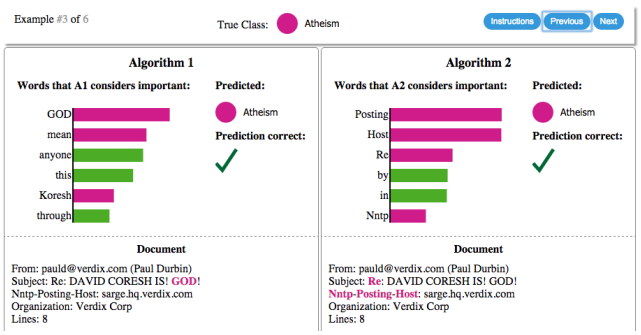
\includegraphics[width=0.75\textwidth]{imagens/lime_exemplo.png}
    \caption{Exemplo de explicação gerada pelo LIME}
    \label{fig:lime_exemplo}
    \legend{Fonte: \citeonline{ribeiro2016}}
\end{figure}

% - - - - - - - - - - - - - - - - - - - - - - - - - - - - - - -
\subsubsection{Aplicação em classificação de texto}
\label{subsubsec:lime_texto}

No contexto de classificação de texto, cada palavra (ou \textit{token}) da entrada é tratada como uma \textit{feature}, ou seja, uma característica binária que indica se está presente ou ausente no texto. A explicação LIME indica quais palavras, quando presentes, aumentam a probabilidade de cada classe, e quais palavras a diminuem. O resultado pode ser visualizado como um destaque colorido sobre o texto original, onde palavras em verde contribuem positivamente para a classe predita e palavras em vermelho contribuem negativamente \cite{mustafa2025}.

\citeonline{mustafa2025} demonstraram que a aplicação de LIME na 
classificação de texto não apenas produz explicações úteis para o 
usuário final, mas também contribui para melhorar o processo de 
pré-processamento: ao revelar que \textit{stopwords} recebem pesos 
desproporcionalmente altos nas explicações, o LIME evidenciou a 
necessidade de sua remoção.

% - - - - - - - - - - - - - - - - - - - - - - - - - - - - - - -
\subsubsection{Vantagens e limitações}
\label{subsubsec:lime_limitacoes}

A principal vantagem do LIME é sua generalidade: o método funciona com qualquer modelo e qualquer tipo de entrada sem necessidade de acesso ao interior do modelo. Isso o torna especialmente adequado para modelos de caixa-preta como o BERT, cujos mecanismos internos são de difícil interpretação direta.

Sua principal limitação é a instabilidade das explicações. Por 
depender de amostragem aleatória de perturbações, execuções diferentes 
do LIME sobre a mesma instância podem produzir explicações distintas, 
especialmente quando há colinearidade entre as \textit{features}, 
ou seja, quando algumas características extraídas do texto são muito 
parecidas ou carregam informações semelhantes \cite{salih2023}. Para 
mitigar essa instabilidade, recomenda-se executar o LIME múltiplas 
vezes e analisar a consistência das explicações, ou fixar a semente 
aleatória para garantir reprodutibilidade.

% ---------------------------------------------------------------
\subsection{SHAP — \textit{SHapley Additive exPlanations}}
\label{subsec:shap}

% - - - - - - - - - - - - - - - - - - - - - - - - - - - - - - -
\subsubsection{Fundamentos — valores de Shapley da teoria dos jogos}
\label{subsubsec:shap_fundamentos}

SHAP foi proposto por \citeonline{lundberg2017} com base nos valores 
de Shapley da teoria dos jogos cooperativos. O problema que o SHAP 
resolve é: dada uma predição específica de um modelo, como distribuir 
o ``crédito'' por essa predição de forma justa entre as 
\textit{features} de entrada?

Na teoria dos jogos, o valor de Shapley de um jogador em um jogo 
cooperativo é calculado como a média ponderada de quanto cada jogador 
contribuiu individualmente em todas as combinações possíveis com os 
demais jogadores. \citeonline{lundberg2017} adaptam esse conceito 
para o contexto de modelos de aprendizado de máquina: cada 
\textit{feature} é um ``jogador'', a predição do modelo é o 
``valor do jogo'', e o valor SHAP de cada \textit{feature} mede 
o quanto ela contribuiu para a predição, considerando todas as 
possíveis ordens em que as \textit{features} poderiam ser incluídas.

Formalmente, o valor de Shapley de uma \textit{feature} $i$ 
é calculado como:

\begin{equation}
\phi_i = \sum_{S \subseteq F \setminus \{i\}} 
\frac{|S|!(|F| - |S| - 1)!}{|F|!} 
\left[ f_{S \cup \{i\}}(x_{S \cup \{i\}}) - f_S(x_S) \right]
\end{equation}

onde $F$ é o conjunto de todas as \textit{features}, $S$ é um 
subconjunto que não inclui $i$, $f(S)$ é a predição do modelo 
usando apenas as \textit{features} em $S$, e 
$f(S \cup \{i\})$ é a predição incluindo a \textit{feature} 
$i$ \cite{lundberg2017}. O fator 
$\frac{|S|!(|F| - |S| - 1)!}{|F|!}$ garante que todas as 
ordenações possíveis de inclusão das \textit{features} sejam 
consideradas com peso igual, assegurando a propriedade de 
simetria.

A Figura~\ref{fig:shap_exemplo} ilustra esse conceito: cada 
\textit{feature} desloca a predição do valor base até o 
valor final do modelo.

\begin{figure}[H]
    \centering
    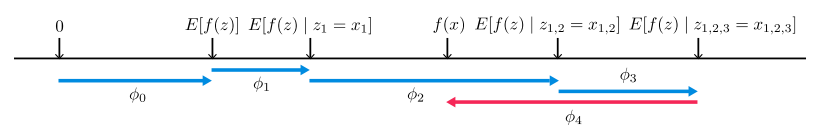
\includegraphics[width=0.75\textwidth]{imagens/shap_exemplo.png}
    \caption{Representação dos valores SHAP por \textit{feature}}
    \label{fig:shap_exemplo}
    \legend{Fonte: \citeonline{lundberg2017}}
\end{figure}

% - - - - - - - - - - - - - - - - - - - - - - - - - - - - - - -
\subsubsection{Propriedades matemáticas — eficiência, simetria e ausência}
\label{subsubsec:shap_propriedades}

A formulação baseada em valores de Shapley garante ao SHAP três propriedades matemáticas desejáveis que o distinguem de métodos \textit{ad hoc} de atribuição de importância \cite{lundberg2017}. A propriedade de eficiência estabelece que a soma dos valores SHAP de todas as \textit{features} iguala a diferença entre a predição do modelo para a instância em questão e o valor base (predição média do modelo sobre o conjunto de dados). A propriedade de simetria estabelece que \textit{features} com contribuições iguais ao modelo recebem valores SHAP iguais, independentemente de sua posição na entrada. A propriedade de ausência estabelece que \textit{features} que não afetam a predição recebem valor SHAP zero.

Essas propriedades conferem ao SHAP uma fundamentação teórica sólida que o LIME não possui, tornando suas explicações mais consistentes e matematicamente justificáveis.

% - - - - - - - - - - - - - - - - - - - - - - - - - - - - - - -
\subsubsection{\textit{KernelSHAP} e aplicação em modelos de texto}
\label{subsubsec:shap_kernel}

Calcular o valor exato de Shapley se torna inviável quando o modelo 
possui muitas \textit{features}, pois seria necessário testar todas 
as combinações possíveis entre elas, o que cresce exponencialmente. 
Para resolver isso, o \textit{KernelSHAP} \cite{lundberg2017} estima 
esses valores testando apenas uma amostra dessas combinações, tornando 
o método viável mesmo em modelos de texto, onde cada \textit{token} 
é tratado como uma \textit{feature}.

Para modelos baseados em \textit{transformers}, o \textit{KernelSHAP} é a variante mais utilizada. O resultado é um vetor de importância por \textit{token} que pode ser visualizado como mapa de calor sobre o texto de entrada, \textit{tokens} com valores SHAP positivos contribuem para a classe predita, e \textit{tokens} com valores negativos contribuem contra ela. O presente trabalho, pretende utilizar esses valores SHAP por token como pesos dos nós no grafo de co-ocorrência proposto.
% ---------------------------------------------------------------
\subsection{Comparação entre SHAP e LIME}
\label{subsec:shap_lime}

% - - - - - - - - - - - - - - - - - - - - - - - - - - - - - - -
\subsubsection{Consistência e estabilidade das explicações}
\label{subsubsec:comparacao_consistencia}

\citeonline{salih2023} realizaram uma análise comparativa abrangente entre SHAP e LIME, avaliando suas propriedades teóricas e comportamento empírico em tarefas de classificação. Em termos de consistência, o SHAP demonstra maior estabilidade: por ser baseado em uma formulação matemática única com garantias teóricas, suas explicações são menos sensíveis à aleatoriedade do processo de amostragem. O LIME, por depender de perturbações aleatórias e de um processo de ajuste local, pode produzir explicações distintas para a mesma instância em execuções diferentes.

Os autores concluem que SHAP é preferível quando a consistência e a fundamentação teórica das explicações são prioritárias, enquanto o LIME pode ser preferível quando a velocidade de geração das explicações é mais importante do que a estabilidade.

% - - - - - - - - - - - - - - - - - - - - - - - - - - - - - - -
\subsubsection{Custo computacional}
\label{subsubsec:comparacao_custo}

Em termos de custo computacional, o LIME é mais eficiente que o 
\textit{KernelSHAP} em textos longos porque trabalha com um número 
fixo de perturbações. Já o \textit{KernelSHAP} exige uma amostragem 
muito maior de combinações de \textit{features} para gerar estimativas 
precisas, o que eleva o tempo de processamento \cite{salih2023}. 
Para textos curtos, como os chamados de suporte de TI, que tipicamente 
contêm poucas dezenas de palavras, essa diferença de custo é menos 
pronunciada.
% - - - - - - - - - - - - - - - - - - - - - - - - - - - - - - -
\subsubsection{Justificativa para uso conjunto neste trabalho}
\label{subsubsec:comparacao_justificativa}

A decisão de implementar e comparar SHAP e LIME neste trabalho, em vez de escolher apenas um dos métodos, é fundamentada em duas razões. Primeiro, a comparação entre os dois métodos produz evidência empírica sobre a qualidade e consistência das explicações geradas para chamados de TI em PT-BR, contribuição metodológica relevante para a literatura sobre XAI em domínios especializados. Segundo, a construção do grafo de co-ocorrência proposto utiliza os valores SHAP como pesos dos nós, mas a comparação com as explicações LIME permite avaliar se a escolha do método de XAI afeta a estrutura e a interpretabilidade do grafo resultante.

% ---------------------------------------------------------------
\subsection{XAI aplicado a classificação de texto e tickets de TI}
\label{subsec:xai_aplicado}

% - - - - - - - - - - - - - - - - - - - - - - - - - - - - - - -
\subsubsection{LIME em classificação multiclasse de texto}
\label{subsubsec:xai_mustafa}

\citeonline{mustafa2025} propuseram um \textit{framework} de 
classificação de texto que combina PLN e XAI. O sistema inclui 
pré-processamento com NLTK (\textit{Natural Language Toolkit}), 
balanceamento de classes com SMOTE (\textit{Synthetic Minority 
Oversampling Technique}) para lidar com datasets desbalanceados, 
e validação cruzada estratificada repetida: uma técnica que divide 
os dados em múltiplos subconjuntos para avaliar o modelo de forma 
mais robusta, garantindo que todas as classes estejam representadas 
em cada divisão. O modelo utilizado foi um híbrido de regressão 
\textit{ridge} com regressão logística. O LIME foi utilizado para 
validar a explicabilidade das classificações em seis domínios 
distintos: medicina, esportes, entretenimento, política, tecnologia 
e negócios. O modelo híbrido atingiu 99\% de acurácia após a 
aplicação do pré-processamento informado pelas explanações LIME.

O trabalho demonstra que a integração de XAI ao \textit{pipeline} 
de classificação não é apenas uma camada de interpretabilidade 
adicionada ao final do processo, mas pode também influenciar 
decisões de pré-processamento e seleção de \textit{features}, 
melhorando a qualidade do modelo como um todo.

% - - - - - - - - - - - - - - - - - - - - - - - - - - - - - - -
\subsubsection{SHAP e LIME em ambiente ITSM corporativo}
\label{subsubsec:xai_razma}

\citeonline{razma2026} aplicaram LIME e SHAP em um ambiente ITSM corporativo real, comparando as explicações geradas para o modelo de regressão logística com \textit{TF-IDF} e para o mBERT \textit{fine-tuned}. Os resultados qualitativos das explicações foram significativamente distintos: o modelo linear tendia a destacar palavras-chave literais com alta frequência no corpus, enquanto o BERT destacava termos semanticamente coerentes com o significado do chamado.

Essa diferença qualitativa nas explicações, documentada por 
\citeonline{razma2026}, sugere que o BERTimbau, combinado com SHAP 
e LIME, tende a produzir explicações mais acuradas em termos de 
importância de \textit{features} e potencialmente mais interpretáveis 
para analistas de TI sem formação em aprendizado de máquina, hipótese que será verificada empiricamente no presente trabalho, 
avaliando se os termos destacados fazem sentido para cada categoria 
de chamado classificada.

% ===============================================================
\section{Grafos de Co-ocorrência como Representação Estrutural de Texto}
\label{sec:grafos}

% ---------------------------------------------------------------
\subsection{Fundamentos de grafos aplicados a texto}
\label{subsec:grafos_fundamentos}

% - - - - - - - - - - - - - - - - - - - - - - - - - - - - - - -
\subsubsection{Definição de grafo de co-ocorrência — nós, arestas e janela deslizante}
\label{subsubsec:grafos_definicao}

Um grafo de co-ocorrência de texto é uma estrutura $G = (V, E)$ onde o conjunto de nós $V$ representa os \textit{tokens} únicos do texto e o conjunto de arestas $E$ conecta pares de \textit{tokens} que co-ocorrem dentro de uma janela deslizante de tamanho $w$ sobre o texto. A janela deslizante percorre o texto posição por posição; em cada posição, todos os pares de \textit{tokens} dentro da janela recebem uma aresta ou têm o peso de sua aresta existente incrementado \cite{yao2019}.

Essa representação captura informação estrutural sobre o texto que as representações vetoriais não preservam: dois \textit{tokens} que frequentemente aparecem juntos no mesmo contexto estarão conectados por uma aresta de alto peso no grafo, independentemente de sua posição absoluta na sequência. Para chamados de TI, isso significa que termos técnicos que tendem a co-ocorrer em chamados de uma mesma categoria, como ``VPN'' e ``acesso'' em chamados de conectividade, estarão estruturalmente próximos no grafo.

% - - - - - - - - - - - - - - - - - - - - - - - - - - - - - - -
\subsubsection{Ponderação de arestas — frequência, PMI e TF-IDF}
\label{subsubsec:grafos_ponderacao}

O peso das arestas em um grafo de co-ocorrência pode ser determinado por diferentes métricas. A abordagem mais simples utiliza a frequência bruta de co-ocorrência, ou seja, a contagem de quantas vezes o par de \textit{tokens} co-ocorreu dentro da janela deslizante. Métricas mais sofisticadas, como a Informação Mútua Pontual (PMI, do inglês \textit{Pointwise Mutual Information}), normalizam a frequência de co-ocorrência pelas frequências individuais de cada \textit{token}, favorecendo pares que co-ocorrem mais do que seria esperado pelo acaso \cite{yao2019}.

No presente trabalho, os pesos das arestas serão determinados pela frequência de co-ocorrência normalizada, enquanto os pesos dos \textit{nós}, que constituem o elemento central da proposta, serão determinados pelos valores SHAP calculados para cada \textit{token} pelo modelo BERTimbau. Essa distinção entre ponderação de arestas (estrutura relacional) e ponderação de nós (relevância explicativa) é a inovação central da camada de visualização proposta.

% ---------------------------------------------------------------
\subsection{\textit{TextGCN} — formalização do grafo de co-ocorrência}
\label{subsec:textgcn}

% - - - - - - - - - - - - - - - - - - - - - - - - - - - - - - -
\subsubsection{Grafo heterogêneo documento-palavra}
\label{subsubsec:textgcn_grafo}

\citeonline{yao2019} propuseram o \textit{TextGCN} (\textit{Text Graph Convolutional Network}), modelo que constrói um único grafo heterogêneo para todo o corpus, conectando documentos e palavras. As arestas documento-palavra recebem pesos baseados em TF-IDF, refletindo a importância de cada palavra para cada documento. As arestas palavra-palavra recebem pesos baseados em PMI calculada sobre co-ocorrências em janela deslizante de tamanho 20 sobre todo o corpus, refletindo a força de associação semântica entre pares de palavras.

Essa estrutura permite que as redes neurais de grafos (GCN) propaguem informação simultaneamente entre documentos e palavras, capturando relações semânticas globais que modelos baseados em sequências não conseguem representar diretamente.

% - - - - - - - - - - - - - - - - - - - - - - - - - - - - - - -
\subsubsection{Redes neurais de grafos e propagação de informação}
\label{subsubsec:textgcn_gcn}

As redes neurais de grafos (GNN, do inglês \textit{Graph Neural Networks}) operam sobre grafos propagando informação entre nós vizinhos por meio de operações de agregação e transformação. Em cada camada da rede, a representação de cada nó é atualizada com base nas representações de seus vizinhos na iteração anterior \cite{yao2019}. Após múltiplas camadas, cada nó possui uma representação que agrega informação de sua vizinhança local de múltiplos saltos.

No contexto deste trabalho, a relevância do \textit{TextGCN} é fundamentalmente teórica: ele formaliza matematicamente a estrutura do grafo de co-ocorrência e demonstra sua utilidade para classificação de texto. O presente trabalho não irá implementar GCN, o grafo de co-ocorrência será utilizado exclusivamente como estrutura de visualização para as explanações XAI, não como componente do modelo de classificação.

% ---------------------------------------------------------------
\subsection{Combinação de BERT com grafos de co-ocorrência}
\label{subsec:bert_grafo}

% - - - - - - - - - - - - - - - - - - - - - - - - - - - - - - -
\subsubsection{\textit{Embeddings} BERT como \textit{features} iniciais dos nós}
\label{subsubsec:bert_grafo_embeddings}

\citeonline{yang2021} propuseram o BEGNN (\textit{BERT-Enhanced Graph Neural Network}), que combina representações contextualizadas do BERT com grafos de co-ocorrência para classificação de texto. Na arquitetura BEGNN, o BERT gera \textit{embeddings} contextualizados para cada \textit{token} da entrada; esses \textit{embeddings} são utilizados como \textit{features} iniciais dos nós do grafo de co-ocorrência correspondente ao documento. Em seguida, uma GCN propaga informação entre nós vizinhos, produzindo representações enriquecidas pela estrutura do grafo. A representação final do documento é obtida por agregação das representações dos nós.

Essa combinação aborda uma limitação do BERT quando utilizado isoladamente: o mecanismo de atenção do BERT captura relações entre \textit{tokens}, mas essas relações são implícitas nos pesos de atenção e não explicitamente estruturadas como um grafo. O grafo de co-ocorrência fornece uma estrutura explícita que complementa as representações contextualizadas.

% - - - - - - - - - - - - - - - - - - - - - - - - - - - - - - -
\subsubsection{Resultados em vocabulário técnico especializado}
\label{subsubsec:bert_grafo_resultados}

\citeonline{yang2021} avaliaram o BEGNN em múltiplos \textit{datasets} de classificação de texto, demonstrando que a combinação BERT + grafo supera tanto o BERT isolado quanto o \textit{TextGCN}, especialmente em \textit{datasets} com vocabulário técnico especializado. Esse resultado é relevante para o presente trabalho porque chamados de suporte de TI são exatamente o tipo de texto com vocabulário técnico especializado para o qual o BEGNN demonstrou vantagem, sugerindo que a estrutura de grafo de co-ocorrência captura informação complementar às representações do BERTimbau.

% ---------------------------------------------------------------
\subsection{Grafo de co-ocorrência combinado com XAI}
\label{subsec:grafo_xai}

% - - - - - - - - - - - - - - - - - - - - - - - - - - - - - - -
\subsubsection{Ponderação de nós por \textit{scores} de explicabilidade}
\label{subsubsec:grafo_xai_ponderacao}

\citeonline{talebi2025} apresentam o trabalho de maior proximidade 
metodológica com o presente TCC: aplicam RoBERTa combinado com LIME 
e um grafo de co-ocorrência para detectar \textit{body shaming}, 
prática de humilhar pessoas com base em sua aparência física, em 
redes sociais em inglês. No trabalho de Talebi e Abdolvand, o grafo 
de co-ocorrência é construído com nós representando \textit{tokens} 
e arestas ponderadas pelos \textit{scores} LIME de cada \textit{token}. 
Os \textit{tokens} com maior importância LIME produzem arestas de 
maior peso com seus vizinhos na janela de co-ocorrência.

O presente trabalho adotará uma abordagem estruturalmente análoga, 
mas com diferenças importantes: utilizará BERTimbau em vez de 
RoBERTa, aplicará os valores SHAP como pesos dos nós em vez dos 
\textit{scores} LIME como pesos de arestas, e o domínio de aplicação 
será a classificação de chamados de suporte de TI em português 
brasileiro. A escolha de ponderar os nós em vez das arestas reflete 
a intenção de destacar visualmente os \textit{tokens} individualmente 
mais relevantes para a predição, enquanto as arestas manterão sua 
função de representar a estrutura de co-ocorrência do texto.

% - - - - - - - - - - - - - - - - - - - - - - - - - - - - - - -
\subsubsection{Visualização interativa como camada de auditabilidade}
\label{subsubsec:grafo_xai_visualizacao}

A literatura aponta que a combinação de grafos de co-ocorrência com \textit{scores} de explicabilidade pode ser exibida em interfaces interativas 
que tornam o processo decisório auditável. Nessa abordagem, os nós 
do grafo são dimensionados proporcionalmente à importância de cada 
\textit{token} calculada pelo método XAI, e as arestas são ponderadas 
pela frequência de co-ocorrência, produzindo uma representação visual 
que combina estrutura relacional do texto com relevância explicativa 
do modelo \cite{talebi2025}.

Essa camada de visualização tem o potencial de transformar a saída 
opaca do modelo em uma representação auditável, endereçando diretamente 
o problema identificado por \citeonline{zemp2021} e 
\citeonline{razma2026}: analistas de suporte precisam compreender por 
que o modelo tomou determinada decisão para confiar no sistema e 
adotá-lo em produção. A solução proposta neste trabalho adota essa 
abordagem, cuja implementação é detalhada no Capítulo~\ref{cap:desenvolvimento}.
% ===============================================================
\section{Síntese da Literatura e Posicionamento do Trabalho}
\label{sec:sintese}

% ---------------------------------------------------------------
\subsection{Lacunas identificadas no estado da arte}
\label{subsec:sintese_lacunas}

% - - - - - - - - - - - - - - - - - - - - - - - - - - - - - - -
\subsubsection{Ausência de XAI em sistemas de classificação de tickets em produção}
\label{subsubsec:lacuna_xai}

O trabalho de \citeonline{zemp2021} demonstra que sistemas de classificação de chamados de TI com alta acurácia são tecnicamente viáveis e já foram implantados em produção. No entanto, a ausência de mecanismos de explicabilidade limita a adoção e a auditabilidade desses sistemas. Os agentes de suporte recebem predições sem justificativa, o que dificulta a identificação de erros sistemáticos e a construção de confiança no sistema. Nenhum dos trabalhos de classificação de chamados de TI identificados no screening incorpora uma camada de visualização gráfica para explanações XAI.

% - - - - - - - - - - - - - - - - - - - - - - - - - - - - - - -
\subsubsection{Carência de soluções robustas para PT-BR em \textit{helpdesk}}
\label{subsubsec:lacuna_ptbr}

Os trabalhos de \citeonline{yokota2025} e \citeonline{pereira2023} evidenciam que o estado da arte em classificação de chamados de suporte em português brasileiro ainda é incipiente. Os melhores resultados reportados com modelos simples (75\% de precisão média com ML tradicional e F1-macro insatisfatório com NB e MLP) são inferiores a modelos baseados em \textit{transformers} já alcançados em inglês. Não foi identificado nenhum trabalho nacional que aplique BERTimbau com XAI a chamados de suporte de TI.

% - - - - - - - - - - - - - - - - - - - - - - - - - - - - - - -
\subsubsection{Custo-benefício do BERT sem camada de explicabilidade}
\label{subsubsec:lacuna_wahba}

\citeonline{wahba2023} questiona o uso de BERT para classificação de texto em domínios especializados, argumentando que o custo computacional adicional não se justifica diante da pequena vantagem sobre o SVM em textos técnicos com baixa polissemia. Esse argumento permanece válido enquanto o único critério de avaliação for a acurácia. O presente trabalho responde a esse argumento propondo que o custo do BERTimbau se justifica quando a camada de XAI e grafo de co-ocorrência é adicionada, transformando a saída opaca do modelo em algo auditável e confiável para os analistas, critério que modelos lineares não conseguem satisfazer com a mesma qualidade de explanação.

% ---------------------------------------------------------------
\subsection{Direcionamento para a proposta}
\label{subsec:sintese_direcao}

Diante das lacunas identificadas: ausência de XAI em sistemas de classificação de chamados em produção, carência de soluções robustas para PT-BR em \textit{helpdesk} de TI, e a questão do custo-benefício do BERT sem explicabilidade, o presente trabalho propõe um \textit{pipeline} que combina BERTimbau, SHAP, LIME e grafo de co-ocorrência ponderado para classificação de chamados em PT-BR com explicabilidade visual. A descrição detalhada da arquitetura, do \textit{dataset}, dos experimentos e da interface que será desenvolvida é apresentada no Capítulo~\ref{cap:desenvolvimento}.

% ---------------------------------------------------------------
\section{Metodologia da pesquisa bibliográfica}
\label{sec:metodologia_pesquisa}

A pesquisa bibliográfica foi realizada nas bases Google Scholar, IEEE Xplore, arXiv e SciELO, utilizando as palavras-chave ``BERT'', ``Grafos'', ``XAI'', ``PLN'', ``Help Desk'', ``Chamados de TI'', ``SHAP'', ``LIME'', ``Tickets'', ``Support'', ``Pipeline'', ``Classificação'', ``Caixa Preta'' e ``Knowledge Graph'', entre outras. Foram selecionados artigos publicados entre 2021 e 2026, em português e inglês, que tivessem relação direta com o tema abordado.

% ---------------------------------------------------------------
\section{Fundamentos}
\label{sec:fundamentos}
 
Esta seção apresenta os conceitos técnicos fundamentais que sustentam a proposta deste trabalho. O objetivo é fornecer ao leitor as definições necessárias para compreender a solução proposta antes de sua descrição detalhada.
 
% - - - - - - - - - - - - - - - - - - - - - - - - - - - - - - -
\subsection{Processamento de Linguagem Natural}
 
Processamento de Linguagem Natural (PLN) é o campo da inteligência artificial dedicado ao desenvolvimento de métodos computacionais para compreender, interpretar e gerar linguagem humana. No contexto deste trabalho, PLN é utilizado para representar chamados de suporte técnico como vetores numéricos que um modelo de aprendizado de máquina possa processar, e para extrair informações semânticas dos textos submetidos pelos usuários \cite{devlin2019}.
 
% - - - - - - - - - - - - - - - - - - - - - - - - - - - - - - -
\subsection{Modelos de Linguagem Baseados em \textit{Transformer}}
 
Modelos de linguagem baseados na arquitetura \textit{Transformer} \cite{vaswani2017} aprendem representações contextualizadas de texto por meio de mecanismos de atenção que consideram simultaneamente todas as posições de uma sequência de entrada. O BERT \cite{devlin2019} é o modelo desta família mais amplamente adotado para tarefas de classificação de texto. O BERTimbau \cite{souza2020} é uma variante do BERT pré-treinada especificamente sobre corpora em português brasileiro, sendo o modelo adotado neste trabalho.
 
% - - - - - - - - - - - - - - - - - - - - - - - - - - - - - - -
\subsection{Inteligência Artificial Explicável}
 
Inteligência Artificial Explicável (XAI) refere-se ao conjunto de métodos e técnicas que permitem compreender e auditar as decisões de modelos de aprendizado de máquina \cite{salih2023}. Dois métodos \textit{post-hoc} serão utilizados neste trabalho:
 
\begin{itemize}
    \item \textbf{LIME} \cite{ribeiro2016}: explica predições individuais ajustando um modelo linear simples em torno de perturbações da entrada original, indicando quais palavras mais contribuíram para a classificação.
 
    \item \textbf{SHAP} \cite{lundberg2017}: atribui a cada palavra da entrada um valor de importância calculado com base na teoria dos jogos cooperativos, com garantias matemáticas de consistência e equidade na distribuição de crédito.
\end{itemize}
 
% - - - - - - - - - - - - - - - - - - - - - - - - - - - - - - -
\subsection{Grafo de Co-ocorrência}
 
Um grafo de co-ocorrência é uma estrutura $G = (V, E)$ na qual os nós $V$ representam os termos únicos de um texto e as arestas $E$ conectam pares de termos que aparecem juntos dentro de uma janela deslizante de tamanho fixo \cite{yao2019}. Neste trabalho, essa estrutura será utilizada como camada de visualização das explicações XAI: os pesos dos nós serão determinados pelos valores SHAP de cada \textit{token}, e os pesos das arestas pela frequência de co-ocorrência, produzindo uma representação visual que combina estrutura relacional do texto com relevância explicativa do modelo.
 
% - - - - - - - - - - - - - - - - - - - - - - - - - - - - - - -
\subsection{Sistema de \textit{Help Desk} e Triagem de Chamados}
 
Um sistema de \textit{help desk} é uma plataforma que centraliza e gerencia solicitações de suporte técnico submetidas pelos usuários de uma organização. A triagem de chamados consiste em classificar cada solicitação em uma categoria predefinida e encaminhá-la à equipe responsável pela resolução. A automação desse processo, substituindo ou auxiliando a triagem manual, é o problema central abordado por este trabalho \cite{zemp2021}.

% ---------------------------------------------------------------
\section{Trabalhos relacionados}
\label{sec:trabalhos_relacionados}

Esta seção analisa três trabalhos que enfrentaram o desafio de automatizar a triagem de chamados de suporte de TI, servindo de base comparativa para a evolução proposta neste TCC.

\subsection{Trabalho 1: Ticket Automation: An Insight into Current Research}

\citeonline{zemp2021} abordou o problema da triagem automática num ambiente corporativo com mais de um milhão de chamados. Para resolvê-lo, o autor comparou modelos CNN, BiLSTM e RoBERTa. A metodologia envolveu o treino em larga escala num \textit{dataset} real de um banco suíço. Os resultados mostraram uma acurácia de 92\%. No entanto, a solução apresentou limitações na aceitação pelos utilizadores finais devido à natureza de "caixa-preta" do modelo. O presente trabalho diferencia-se por focar na explicabilidade via SHAP e Grafos, permitindo que os analistas de TI entendam o "porquê" da classificação.

\subsection{Trabalho 2: Machine Learning for Classification of IT Support Tickets}

\citeonline{wahba2023} enfrentou o mesmo desafio de classificação de \textit{tickets}, mas propôs uma abordagem focada em eficiência para domínios especializados. A solução utilizou um modelo híbrido (HOOM) que combina SVM linear com classificadores \textit{online}. A metodologia demonstrou que em textos técnicos, modelos mais simples podem ser competitivos. Os resultados mostraram boa performance com baixo custo computacional. A limitação identificada é que essa abordagem perde as nuances contextuais que modelos baseados em \textit{Transformers} capturam. O presente trabalho propõe o uso do BERTimbau, específico para PT-BR, combinado com visualização de grafos para suprir a falta de contexto de modelos lineares.

\subsection{Trabalho 3: Classificação hierárquica de textos aplicado ao contexto chamados de suporte}

\citeonline{yokota2025} investigou a classificação de chamados especificamente em português brasileiro, utilizando modelos clássicos como \textit{Naive Bayes} e MLP. A metodologia focou na estrutura hierárquica das categorias de TI. Os resultados apresentaram F1-macro insatisfatório para uso em produção. A lacuna principal foi a incapacidade de modelos simples lidarem com o jargão técnico do suporte em português. O presente trabalho diferencia-se pelo uso de uma arquitetura de estado da arte (BERTimbau) treinada especificamente no nosso idioma, superando as limitações semânticas dos modelos testados por Yokota.

\vspace{0.5cm}

\begin{table}[htb]
    \centering
    \caption{Comparação entre trabalhos relacionados}
    \label{tab:trabalhos_relacionados}
    \resizebox{\textwidth}{!}{
    \begin{tabular}{l|c|c|c|c}
        \toprule
        \textbf{Critério} & \textbf{Zemp (2021)} & \textbf{Wahba (2023)} & 
        \textbf{Yokota (2025)} & \textbf{Este trabalho} \\
        \midrule
        Objetivo & Classificação & Eficiência & Classificação PT-BR & 
        Classificação + XAI \\
        \midrule
        Tecnologia & RoBERTa / CNN & SVM / HOOM & \textit{Naive Bayes} / MLP & 
        BERTimbau + Grafos \\
        \midrule
        Explicabilidade & Não & Intrínseca & Limitada & SHAP / LIME / Grafos \\
        \midrule
        Limitação & Caixa-Preta & Baixo Contexto & Baixa Performance & 
        Custo Computacional \\
        \bottomrule
    \end{tabular}
    }
    \vspace{0.2cm}
    \legend{Fonte: Elaborado pelos autores (2026)}
\end{table}

% ---------------------------------------------------------------
\section{Hipótese de Pesquisa}
\label{sec:hipotese_pesquisa}

A utilização de modelagem em grafos como camada de explicabilidade visual para o modelo BERT aumenta a auditabilidade e a confiança dos gestores de TI no processo de classificação automatizada, mitigando a percepção de 'caixa-preta' sem a necessidade de intervenção manual na triagem.

% ---------------------------------------------------------------
\section{Métricas de Avaliação}
\label{sec:metricas_avaliacao}

A avaliação do desempenho do modelo será realizada por meio de métricas 
amplamente utilizadas em tarefas de classificação textual:

\begin{itemize}
\item \textbf{Acurácia (Accuracy)} – proporção de classificações corretas 
realizadas pelo modelo sobre o total de instâncias avaliadas.

\item \textbf{Precisão (Precision)} – proporção de classificações corretas 
entre os casos previstos para uma determinada categoria, medindo a 
capacidade do modelo de evitar falsos positivos.

\item \textbf{Revocação (Recall)} – capacidade do modelo de identificar 
corretamente os chamados pertencentes a cada categoria, medindo a 
capacidade de evitar falsos negativos.

\item \textbf{F1-score} – média harmônica entre precisão e revocação, 
expressa pela fórmula $F1 = 2 \cdot \frac{Precisão \times Revocação}{Precisão 
+ Revocação}$. Será utilizada a variante \textbf{F1-macro}, que calcula o 
F1-score para cada categoria individualmente e tira a média, tratando todas 
as categorias com peso igual independentemente de seu tamanho, métrica 
especialmente importante em datasets desbalanceados.

\item \textbf{ROC-AUC} (\textit{Receiver Operating Characteristic - Area 
Under the Curve}) – mede a capacidade do modelo de distinguir entre classes 
ao longo de diferentes limiares de decisão. O valor varia entre 0 e 1, sendo 
que 1 representa um classificador perfeito e 0,5 representa um classificador 
aleatório. Em cenários multiclasse, será utilizada a variante 
\textbf{ROC-AUC macro}, que agrega as curvas ROC de cada categoria. Essa 
métrica permite análises complementares, como a avaliação do impacto de 
diferentes combinações de hiperparâmetros sobre a capacidade discriminativa 
do modelo.

\item \textbf{Matriz de confusão} – representação tabular que detalha os 
tipos de erros cometidos pelo modelo durante a classificação, permitindo 
identificar padrões sistemáticos de confusão entre categorias semanticamente 
próximas.
\end{itemize}

% ===============================================================
% CAPÍTULO 3 - DESENVOLVIMENTO
% ===============================================================
%\chapter{Desenvolvimento}
%\label{cap:desenvolvimento}

% Neste capítulo, apresenta-se a solução proposta para o problema identificado, bem como o cronograma de trabalho previsto para o desenvolvimento completo do projeto no TCC2.

% ---------------------------------------------------------------
%\section{Solução proposta}
%\label{sec:solucao}

% Descreva detalhadamente a solução que será desenvolvida para resolver o problema apresentado na introdução. A descrição deve incluir:

% \begin{itemize}
%     \item \textbf{Visão geral da solução}: o que será desenvolvido (sistema, aplicativo, modelo, ferramenta, etc.);
%     \item \textbf{Arquitetura}: como os componentes da solução se organizam e interagem;
%     \item \textbf{Tecnologias e ferramentas}: quais linguagens, frameworks, bibliotecas, bancos de dados e ambientes serão utilizados, e por que foram escolhidos;
%     \item \textbf{Funcionalidades principais}: o que a solução fará para atender aos objetivos;
%     \item \textbf{Metodologia de desenvolvimento}: qual abordagem será utilizada (ágil, cascata, prototipação, etc.);
%     \item \textbf{Critérios de validação}: como será medido o sucesso da solução (métricas, testes, avaliação com usuários, etc.).
% \end{itemize}

% Utilize diagramas, fluxogramas ou mockups para ilustrar a solução. Exemplo de descrição de arquitetura:

% \textit{A solução proposta consiste em uma aplicação web composta por três camadas: front-end desenvolvido em React.js, back-end em Node.js com Express, e banco de dados PostgreSQL. A comunicação entre front-end e back-end será feita por meio de uma API REST.}

% ---------------------------------------------------------------
%\section{Cronograma de trabalho}
%\label{sec:cronograma}

% O cronograma a seguir apresenta, no formato de diagrama de Gantt, as atividades previstas para o desenvolvimento do TCC2, distribuídas ao longo das semanas do semestre.

% \begin{figure}[htb]
%     \centering
%     \caption{Cronograma de atividades -- Diagrama de Gantt}
%     \label{fig:gantt}
%     \begin{ganttchart}[
%         hgrid,
%         vgrid,
%         x unit=0.72cm,
%         y unit title=0.6cm,
%         y unit chart=0.7cm,
%         title height=1,
%         bar height=0.5,
%         bar label font=\scriptsize,
%         title label font=\small,
%         milestone label font=\scriptsize\itshape,
%         group label font=\scriptsize\bfseries,
%         bar/.append style={fill=blue!40},
%         group/.append style={draw=black, fill=blue!70},
%         milestone/.append style={fill=red!70},
%     ]{1}{16}
%         % Título: semanas de 1 a 16
%         \gantttitle{Semanas}{16} \\
%         \gantttitlelist{1,...,16}{1} \\

%         % Grupo 1: Revisão e Planejamento
%         \ganttgroup{Fase 1: Planejamento}{1}{4} \\
%         \ganttbar{Revisão bibliográfica}{1}{3} \\
%         \ganttbar{Definição de requisitos}{2}{4} \\
%         \ganttbar{Projeto da arquitetura}{3}{4} \\
%         \ganttmilestone{Entrega do projeto}{4} \\

%         % Grupo 2: Desenvolvimento
%         \ganttgroup{Fase 2: Desenvolvimento}{5}{11} \\
%         \ganttbar{Implementação do módulo 1}{5}{7} \\
%         \ganttbar{Implementação do módulo 2}{7}{9} \\
%         \ganttbar{Integração dos módulos}{9}{11} \\
%         \ganttmilestone{Protótipo funcional}{11} \\

%         % Grupo 3: Testes e Finalização
%         \ganttgroup{Fase 3: Validação}{12}{16} \\
%         \ganttbar{Testes e validação}{12}{14} \\
%         \ganttbar{Ajustes e correções}{14}{15} \\
%         \ganttbar{Redação final do TCC2}{13}{16} \\
%         \ganttmilestone{Entrega final}{16}

%         % Ligações entre atividades
%         \ganttlink{elem2}{elem3}
%         \ganttlink{elem3}{elem4}
%         \ganttlink{elem4}{elem5}
%         \ganttlink{elem7}{elem8}
%         \ganttlink{elem8}{elem9}
%         \ganttlink{elem9}{elem10}
%         \ganttlink{elem12}{elem13}
%     \end{ganttchart}
%     \legend{Fonte: Elaborado pelo autor (2025)}
% \end{figure}

% \textbf{Instruções para personalização do cronograma}:
% \begin{itemize}
%     \item Ajuste o número de semanas conforme o calendário acadêmico do semestre;
%     \item Modifique as atividades de acordo com as etapas do seu projeto;
%     \item Os marcos (\textit{milestones}) indicam entregas importantes --- adapte-os às datas de avaliação;
%     \item As setas entre atividades indicam dependências --- uma atividade só inicia após a conclusão da anterior;
%     \item Utilize o diagrama como ferramenta de acompanhamento: atualize-o a cada reunião com o orientador.
% \end{itemize}

\chapter{Desenvolvimento}
\label{cap:desenvolvimento}

Neste capítulo, apresenta-se a solução proposta para o problema identificado, bem como o cronograma de trabalho previsto para a implementação completa do projeto no TCC2.

\section{Solução proposta}
\label{sec:solucao}

\subsubsection{Visão geral da solução}

A solução proposta tem como objetivo central classificar 
automaticamente chamados de suporte técnico de forma transparente 
e auditável, utilizando técnicas de Processamento de Linguagem 
Natural (PLN) e Inteligência Artificial Explicável (XAI). O 
diferencial da proposta não é apenas a classificação automática, 
mas a capacidade de explicar cada decisão: o analista poderá 
identificar quais termos do chamado influenciaram a classificação 
e por quê.

Para isso, serão utilizadas duas técnicas complementares de 
explicabilidade: o SHAP, que atribui a cada termo do chamado um 
valor numérico indicando o quanto ele contribuiu para a 
classificação, e o LIME, que gera explicações locais testando 
versões modificadas do texto. Os valores SHAP serão utilizados 
como pesos dos nós em um grafo de co-ocorrência, produzindo uma 
visualização gráfica que combina a estrutura relacional do 
texto com a relevância explicativa de cada termo.

O sistema será desenvolvido para atender principalmente gestores 
e analistas de TI, que poderão utilizá-lo durante o processo de 
triagem para acompanhar de forma transparente e auditável o 
resultado da classificação automática.

% - - - - - - - - - - - - - - - - - - - - - - - - - - - - - - -
\subsection{Protocolo experimental}
\label{subsec:experimentos}

O experimento será estruturado em quatro cenários comparativos, conforme descrito na Tabela~\ref{tab:cenarios}, com o objetivo de isolar a contribuição de cada componente do \textit{pipeline}:

\begin{table}[H]
\centering
\caption{Cenários experimentais para avaliação do sistema}
\label{tab:cenarios}
\begin{tabular}{p{1.5cm} p{3.5cm} p{3.5cm} p{4.5cm}}
\toprule
\textbf{Cenário} & \textbf{Modelo} & \textbf{XAI} & \textbf{Objetivo} \\
\midrule
A & SVM + TF-IDF & Nenhum & Baseline clássico \\
B & BERTimbau & Nenhum & Ganho do transformer \\
C & BERTimbau & SHAP + LIME & Qualidade das explicações \\
D & BERTimbau & SHAP + LIME + grafo & Auditabilidade visual \\
\bottomrule
\end{tabular}
\legend{Fonte: Elaborado pelos autores (2026)}
\end{table}

A comparação entre os cenários A e B avalia o ganho de desempenho do BERTimbau sobre o \textit{baseline} clássico — respondendo ao argumento de \citeonline{wahba2023} sobre o custo-benefício dos \textit{transformers} em domínios especializados. A comparação entre os cenários C e D avalia se a camada de grafo de co-ocorrência oferece auditabilidade superior à exibição isolada de \textit{scores} de importância — hipótese central deste trabalho.

\subsubsection{Protótipos da interface}

Durante a etapa inicial do projeto foram elaborados protótipos de baixa e média fidelidade com o objetivo de validar a organização visual da interface, o fluxo de navegação e a disposição das funcionalidades relacionadas à explicabilidade do modelo.

A etapa de prototipação de baixa fidelidade teve início com a elaboração individual de diferentes propostas de interface por cada integrante do grupo, permitindo que distintas ideias e abordagens fossem exploradas inicialmente. Posteriormente, as principais características de cada proposta foram analisadas e consolidadas em uma versão única do protótipo que passou a servir como base para a continuidade do projeto.

Os protótipos de baixa fidelidade foram utilizados para estruturar os principais componentes da aplicação, definindo a posição dos menus, área de inserção de chamados, painel de resultados e espaço destinado às visualizações explicativas.

\begin{figure}[H]
    \centering
    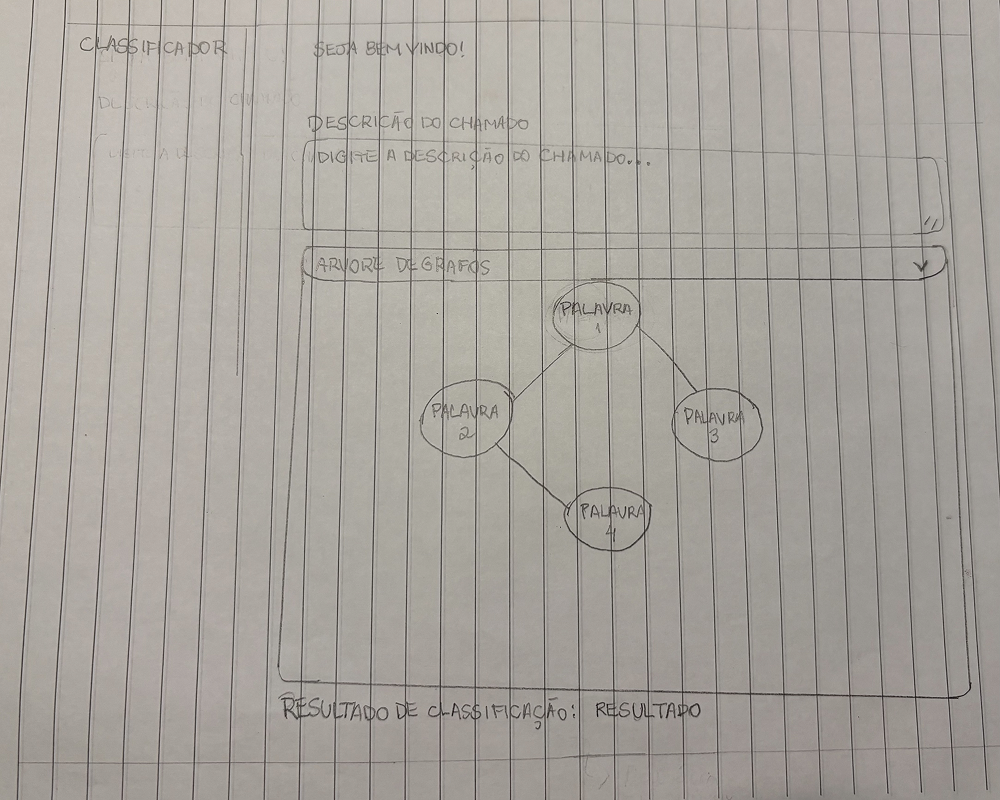
\includegraphics[width=0.75\textwidth]{imagens/baixa_agatha.png}
    \caption{Protótipo de baixa fidelidade da interface por Agatha Barbosa}
    \label{fig:prototipo_baixa_agatha}
\end{figure}

\begin{figure}[H]
    \centering
    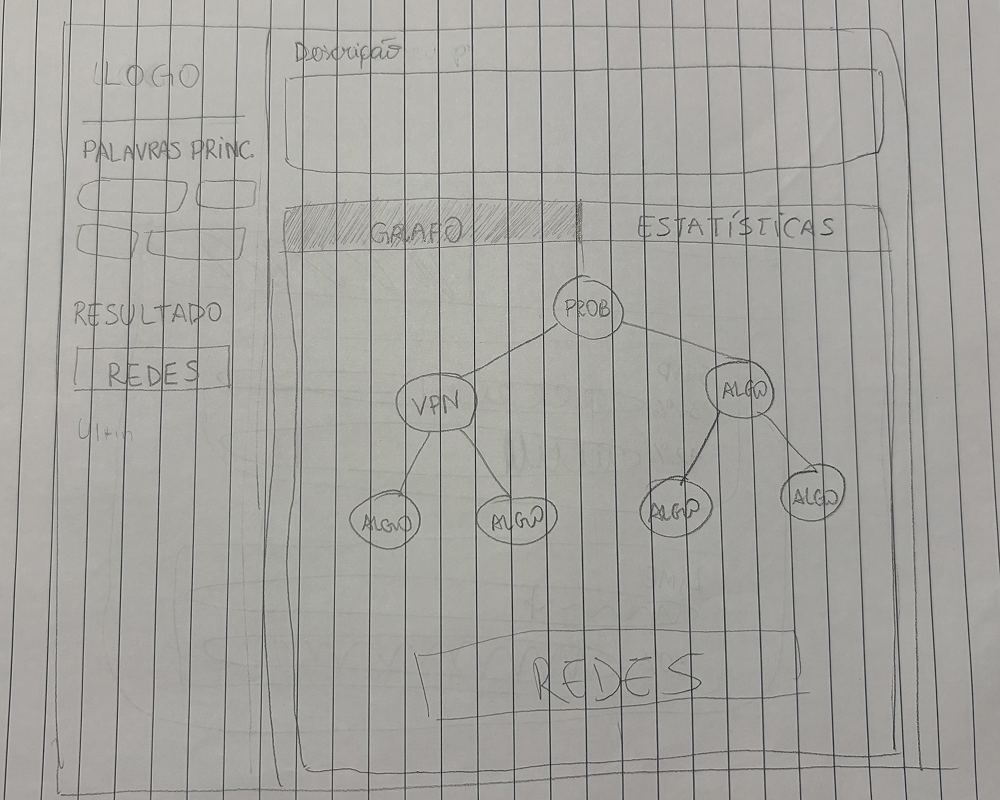
\includegraphics[width=0.75\textwidth]{imagens/baixa_bru.png}
    \caption{Protótipo de baixa fidelidade da interface por Bruna Kinjo}
    \label{fig:prototipo_baixa_bru}
\end{figure}

\begin{figure}[H]
    \centering
    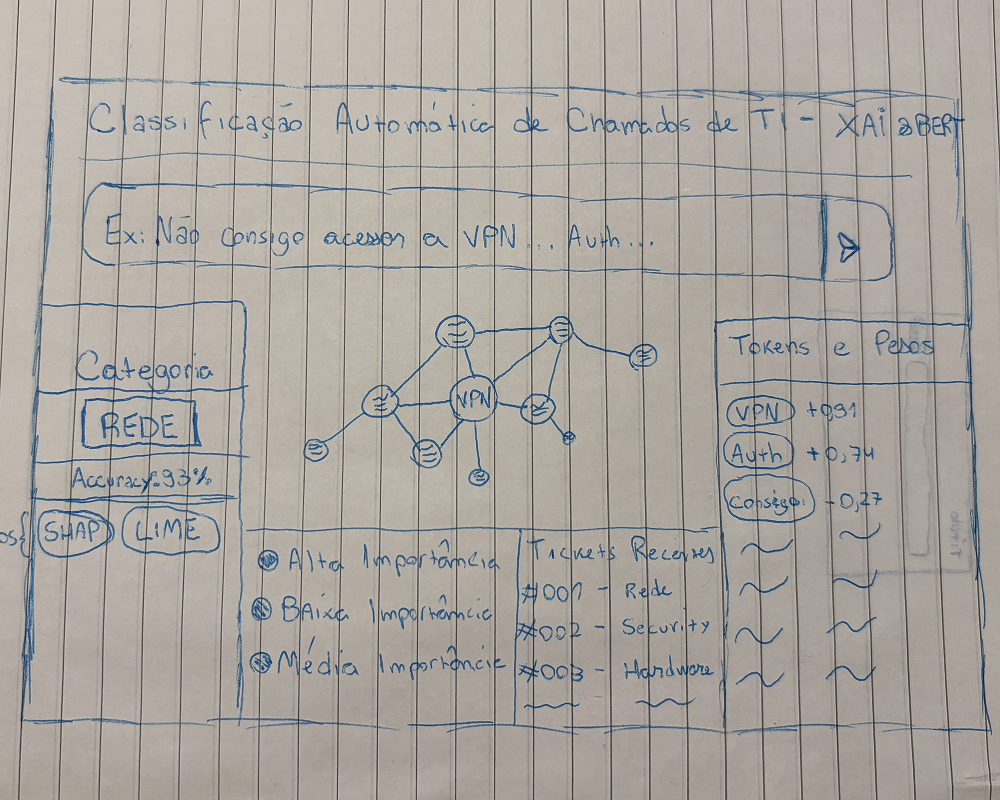
\includegraphics[width=0.75\textwidth]{imagens/baixa_kayke.png}
    \caption{Protótipo de baixa fidelidade da interface por Kayke Ahrens}
    \label{fig:prototipo_baixa_kayke}
\end{figure}

\begin{figure}[H]
    \centering
    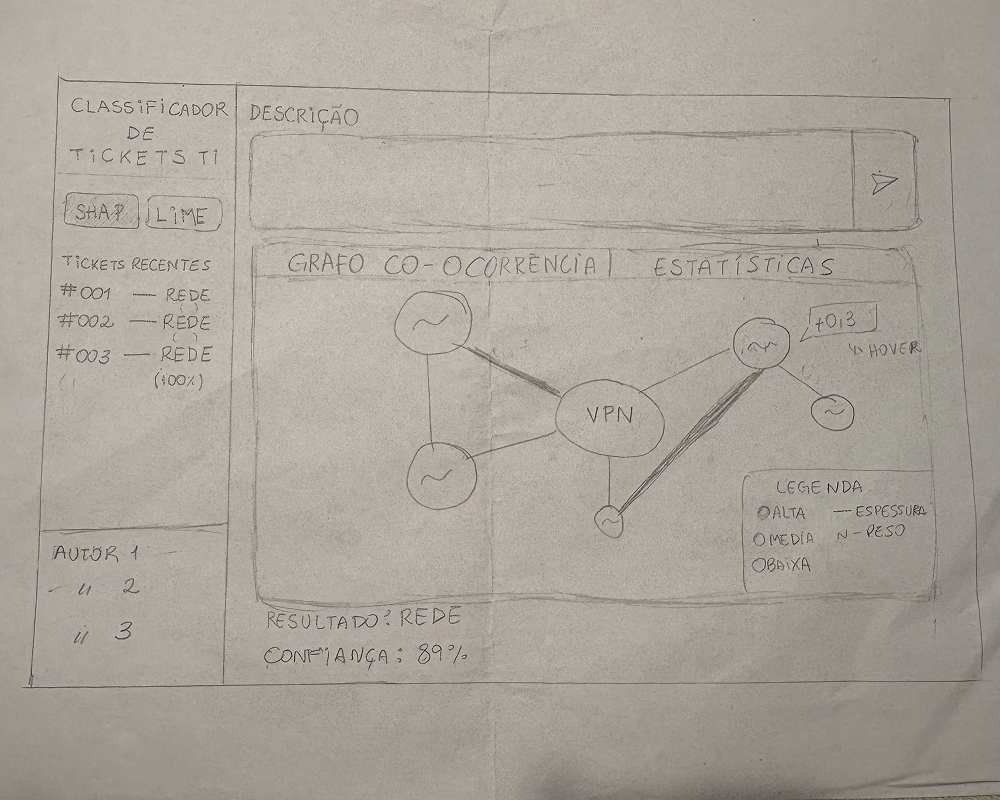
\includegraphics[width=0.75\textwidth]{imagens/baixa_grafo.png}
    \caption{Protótipo de baixa fidelidade da interface final - Tela do grafo}
    \label{fig:prototipo_baixa_grafo}
\end{figure}

\begin{figure}[H]
    \centering
    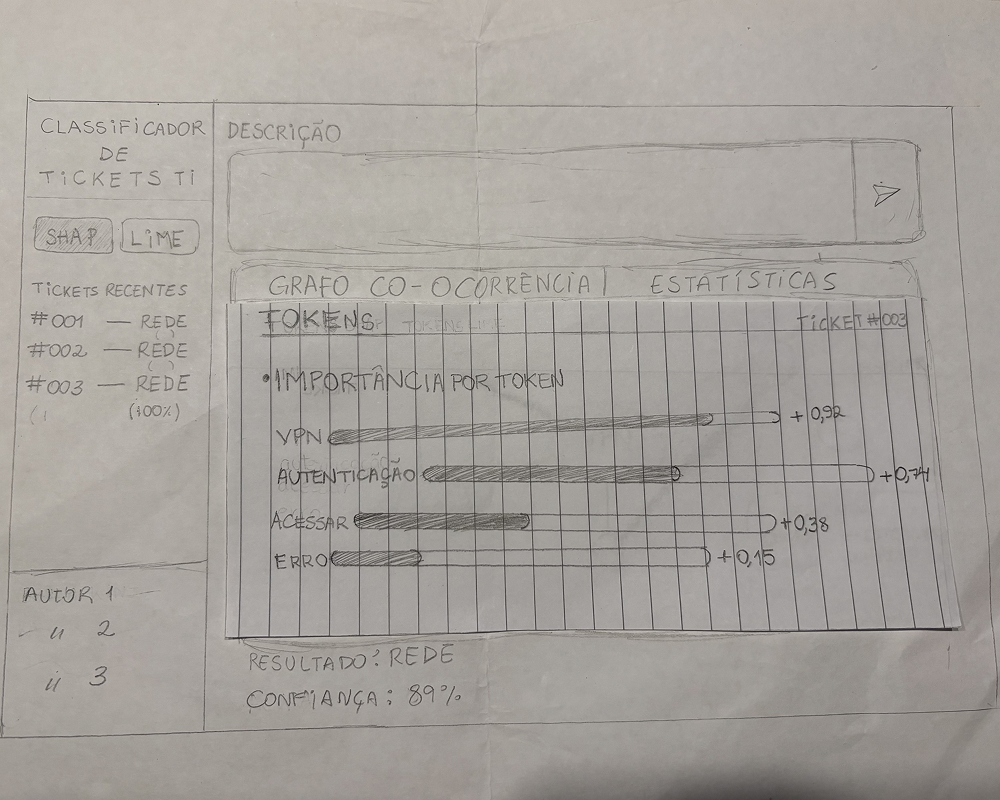
\includegraphics[width=0.75\textwidth]{imagens/baixa_estatisticas.png}
    \caption{Protótipo de baixa fidelidade da interface final - Tela das estatísticas}
    \label{fig:prototipo_baixa_estatisticas}
\end{figure}

Posteriormente, foram elaborados protótipos de média fidelidade com maior nível de detalhamento visual, com foco em validar como as explicações geradas pelo modelo seriam apresentadas de forma compreensível para os analistas de TI. 

A área central do sistema será dedicada às explicações da 
classificação, organizada em duas abas principais, ambas voltadas 
para tornar o processo decisório do modelo auditável:

\begin{itemize}
    \item \textbf{Grafo de Co-Ocorrência}: representação visual das 
    relações entre os \textit{tokens} do chamado, onde o tamanho de 
    cada nó será proporcional ao valor SHAP do termo, indicando sua 
    importância para a classificação, e a espessura das conexões 
    indicará a frequência de co-ocorrência entre os \textit{tokens};
    
    \item \textbf{Estatísticas}: painel que apresentará numericamente 
    a importância individual de cada \textit{token} calculada pelos 
    métodos SHAP e LIME, permitindo ao analista comparar e validar 
    as contribuições de cada termo na decisão do modelo.
\end{itemize}

A escolha por disponibilizar tanto visualizações gráficas quanto 
estatísticas numéricas busca garantir que analistas com diferentes 
perfis consigam auditar as decisões do modelo, seja por meio de 
padrões visuais no grafo ou por comparações quantitativas entre os 
valores de importância dos \textit{tokens}.

Na lateral esquerda do sistema encontra-se a seção ``Tickets 
recentes'', responsável por apresentar classificações realizadas 
anteriormente juntamente com seus respectivos níveis de confiança. 
Esse recurso permitirá consultar rapidamente chamados processados 
anteriormente e auxiliará na análise das classificações realizadas.

Os protótipos desenvolvidos tiveram como principal objetivo verificar 
se os recursos de explicabilidade seriam apresentados de forma 
intuitiva, clara e acessível aos analistas de TI.

\begin{figure}[H]
    \centering
    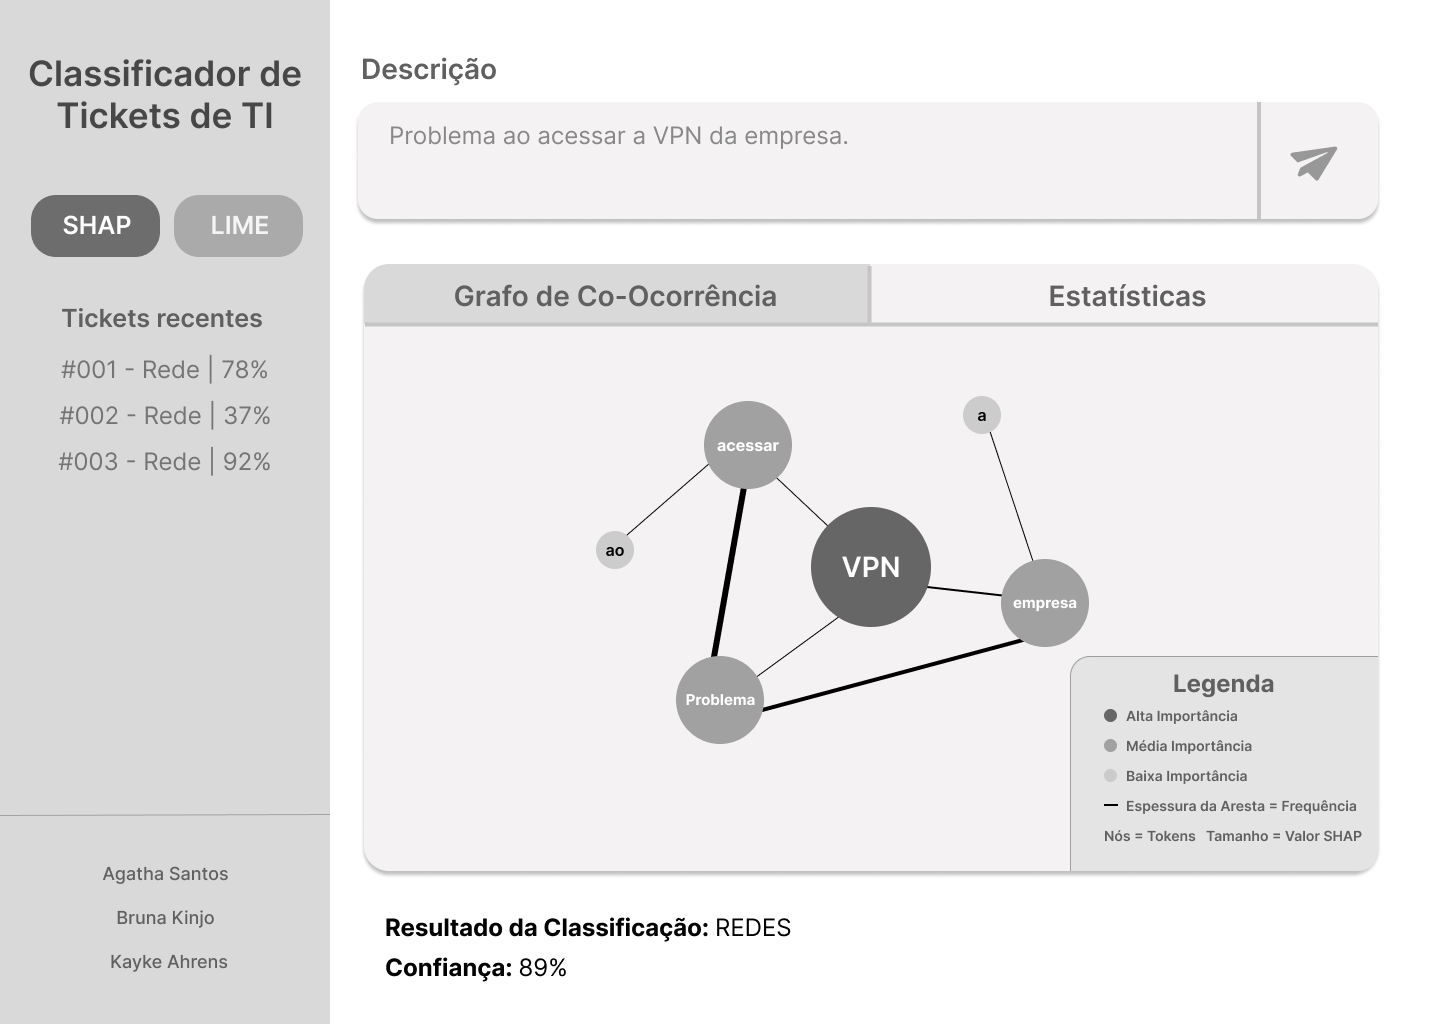
\includegraphics[width=0.75\textwidth]{imagens/grafo.png}
    \caption{Protótipo de média fidelidade - visualização do grafo de co-ocorrência}
    \label{fig:prototipo_media_grafo}
\end{figure}

\begin{figure}[H]
    \centering
    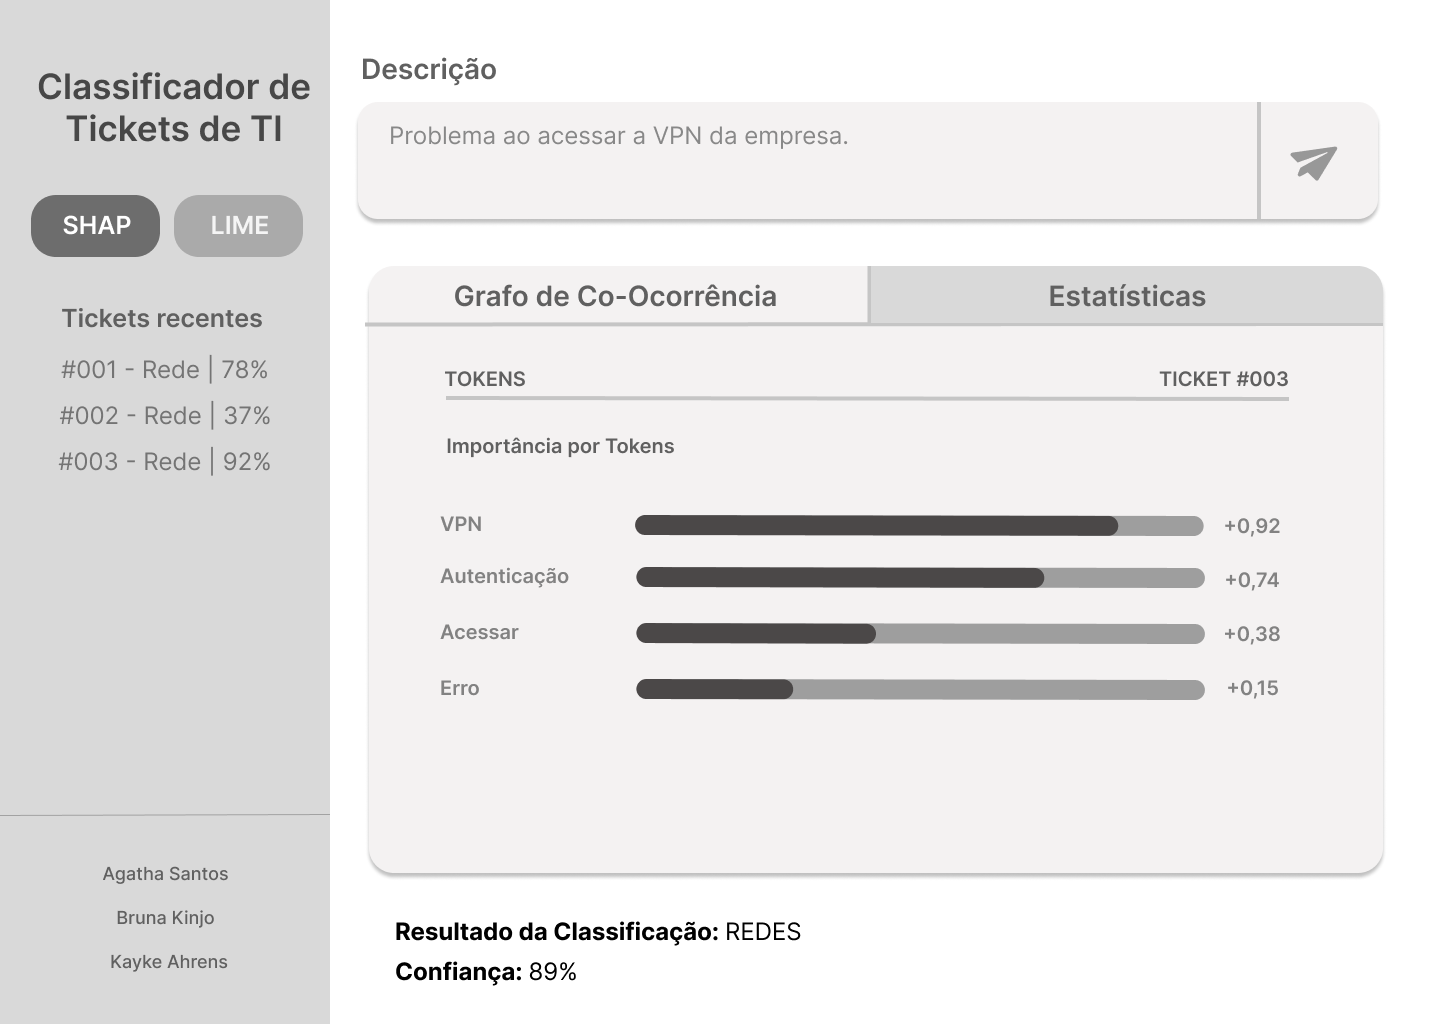
\includegraphics[width=0.75\textwidth]{imagens/estatisticas.png}
    \caption{Protótipo de média fidelidade - visualização estatística dos \textit{tokens}}
    \label{fig:prototipo_media_estatisticas}
\end{figure}

\subsubsection{Arquitetura da solução}

A arquitetura da solução será organizada em três camadas principais:

\begin{itemize}
    \item Camada de apresentação (\textit{front-end});
    \item Camada de processamento;
    \item Camada de dados.
\end{itemize}

A camada de apresentação será responsável pela interação com o usuário final, disponibilizando os formulários de inserção de chamados, exibição das classificações, visualização dos grafos e acesso ao histórico de \textit{tickets} processados.

A camada de processamento será responsável pela execução das etapas de pré-processamento textual, inferência do modelo BERTimbau, cálculo das explicações utilizando SHAP e LIME, além da construção dos grafos de co-ocorrência.

Já a camada de dados será responsável pelo armazenamento das informações relacionadas aos chamados classificados e aos resultados gerados pelo sistema.

O fluxo geral de funcionamento da aplicação seguirá as seguintes etapas:

\begin{enumerate}
    \item \textbf{Pré-processamento} — o texto do chamado é submetido para tokenização, remoção de \textit{stopwords} e normalização. O texto limpo é passado ao tokenizador do BERTimbau, que o converte em \textit{tokens} com seus respectivos IDs e máscaras de atenção.

    \item \textbf{Classificação com BERTimbau} — o modelo BERTimbau com \textit{fine-tuning} processa a sequência de \textit{tokens} e produz, a partir da representação do \textit{token} [CLS], as probabilidades de pertencimento a cada categoria. A categoria com maior probabilidade é selecionada como predição, e o índice de confiança corresponde a essa probabilidade máxima.

    \item \textbf{Cálculo de explicabilidade} — sobre o mesmo texto de entrada, são calculados os valores SHAP e as importâncias LIME. Cada \textit{token} recebe um valor numérico que representa sua contribuição para a predição: valores positivos indicam contribuição para a classe predita, e valores negativos indicam contribuição contrária.

    \item \textbf{Construção do grafo de co-ocorrência} — os \textit{tokens} do chamado são representados como nós de um grafo $G = (V, E)$. As arestas conectam pares de \textit{tokens} que co-ocorrem dentro de uma janela deslizante de tamanho fixo, com pesos proporcionais à frequência de co-ocorrência. Os pesos dos \textbf{nós} são determinados pelos valores SHAP calculados na etapa anterior — \textit{tokens} com maior importância SHAP geram nós visualmente maiores na interface. O grafo é serializado em JSON com a estrutura \texttt{\{nodes, edges\}} e enviado ao \textit{frontend}.

    \item \textbf{Apresentação ao analista} — a interface recebe o JSON, renderiza o grafo e exibe a categoria predita, o índice de confiança, os \textit{tokens} mais relevantes destacados por cor e os valores SHAP e LIME comparativos.
\end{enumerate}

\subsubsection{Tecnologias e ferramentas}

As tecnologias listadas a seguir representam as opções inicialmente 
consideradas para o desenvolvimento do sistema, podendo ser ajustadas 
conforme as decisões técnicas tomadas ao longo da implementação.

\textbf{Interface e visualização:}

\begin{itemize}
    \item React.js; 
    \item CSS;
    \item Biblioteca para visualização de grafos.
\end{itemize}

\textbf{Processamento e Inteligência Artificial:}

\begin{itemize}
    \item Python;
    \item BERTimbau;
    \item SHAP;
    \item LIME;
    \item Bibliotecas de PLN e manipulação de grafos.
\end{itemize}

\textbf{Ambiente de desenvolvimento:}

\begin{itemize}
    \item Git e GitHub;
    \item Jupyter Notebook.
\end{itemize}

\subsubsection{Funcionalidades principais}

Entre as principais funcionalidades previstas para o sistema estão:
%
%\begin{itemize}
%    \item Classificação automática de chamados de TI;
%    \item Exibição da categoria prevista;
%    \item Apresentação do nível de confiança da classificação;
%    \item Visualização da importância dos \textit{tokens} via SHAP e LIME;
%    \item Construção de grafos de co-ocorrência;
%    \item Histórico simplificado de \textit{tickets} classificados;
%    \item Visualização interativa das explicações do modelo.
%\end{itemize}

\begin{itemize}
    \item \textbf{Funcionalidades de explicabilidade:}
    \begin{itemize}
        \item Construção de grafos de co-ocorrência;
        \item Visualização das explicações do modelo.
    \end{itemize}
    \item \textbf{Funcionalidades de classificação e suporte:}
    \begin{itemize}
        \item Classificação automática de chamados de TI;
        \item Exibição da categoria prevista;
        \item Apresentação do nível de confiança da classificação;
        \item Histórico simplificado de \textit{tickets} classificados.
    \end{itemize}
\end{itemize}

\subsubsection{Metodologia de implementação}

A implementação do projeto seguirá uma abordagem iterativa baseada em prototipação e validações incrementais.

Inicialmente foram realizados levantamento bibliográfico, definição dos requisitos e elaboração dos protótipos da interface, etapas já concluídas nesta fase do projeto. Em seguida serão implementados os módulos de classificação automática, explicabilidade e visualização gráfica.

Posteriormente serão realizados testes de integração entre os componentes e ajustes relacionados à usabilidade e apresentação das explicações geradas pelo sistema.

\subsubsection{\textit{Dataset} e \textit{fine-tuning}}

O modelo BERTimbau será ajustado utilizando um conjunto de chamados de dados reais obtidos junto à Bayer Brasil, mediante acordo de confidencialidade e anonimização.

O processo de \textit{fine-tuning} seguirá uma abordagem supervisionada de classificação textual, utilizando divisão entre conjuntos de treino, validação e teste. Também serão aplicadas técnicas de balanceamento de classes e validação de desempenho para reduzir problemas relacionados a \textit{overfitting}, fenômeno que ocorre quando o modelo aprende os dados de treino com precisão excessiva e perde a capacidade de generalizar para novos exemplos, e ao desbalanceamento do \textit{dataset}.

\subsubsection{Critérios de validação}

O sucesso da solução será avaliado sob duas perspectivas complementares.

A primeira perspectiva, \textbf{quantitativa}, avalia o desempenho do modelo de classificação por meio das seguintes métricas: acurácia, precisão, revocação, F1-score macro para lidar com possível desbalanceamento entre categorias, ROC-AUC macro para avaliar a capacidade do modelo de distinguir entre as categorias ao longo de 
diferentes limiares de decisão e matriz de confusão para análise de erros sistemáticos. O BERTimbau será considerado satisfatório se superar o \textit{baseline} SVM em pelo menos 5 pontos percentuais de F1-macro.

A segunda perspectiva, \textbf{qualitativa}, avalia a utilidade das explicações geradas. Serão analisadas: a concordância entre as explicações SHAP e LIME para os mesmos chamados, e a coerência semântica dos \textit{tokens} destacados no grafo em relação à categoria predita — verificando se os termos com maior importância SHAP correspondem intuitivamente ao tipo de problema descrito no chamado.

\section{Cronograma de trabalho}
\label{sec:cronograma}

O cronograma apresentado a seguir organiza as atividades previstas para o TCC2 de forma simplificada.

\begin{figure}[H]
    \centering
    \caption{Cronograma de atividades -- Diagrama de Gantt}
    \label{fig:gantt}
    
    \resizebox{\textwidth}{!}{
        \begin{ganttchart}[
            hgrid,
            vgrid,
            x unit=0.7cm,
            y unit title=0.6cm,
            y unit chart=0.7cm,
            title height=1,
            bar height=0.5,
            bar label font=\scriptsize,
            title label font=\small,
            milestone label font=\scriptsize\itshape,
            group label font=\scriptsize\bfseries,
            bar/.append style={fill=blue!40},
            group/.append style={draw=black, fill=blue!70},
            milestone/.append style={fill=red!70},
            link/.style={->, thick, black}
        ]{1}{16}
            \gantttitle{Semanas}{16} \\
            \gantttitlelist{1,...,16}{1} \\
     
            \ganttgroup{Fase 1: Dados e modelo}{1}{5} \\
            \ganttbar{Obtenção e limpeza do dataset}{1}{2} \\
            \ganttbar{Pré-processamento e balanceamento}{2}{3} \\
            \ganttbar{Fine-tuning do BERTimbau}{3}{5} \\
            \ganttmilestone{Modelo treinado e avaliado}{5} \\
     
            \ganttgroup{Fase 2: XAI e grafo}{5}{9} \\
            \ganttbar{Implementação do SHAP e LIME}{5}{7} \\
            \ganttbar{Construção do grafo de co-ocorrência}{7}{9} \\
            \ganttmilestone{Pipeline XAI funcional}{9} \\
     
            \ganttgroup{Fase 3: Sistema e interface}{9}{13} \\
            \ganttbar{Desenvolvimento da API FastAPI}{9}{11} \\
            \ganttbar{Desenvolvimento do frontend React}{10}{13} \\
            \ganttbar{Integração backend + frontend}{12}{13} \\
            \ganttmilestone{Protótipo funcional completo}{13} \\
     
            \ganttgroup{Fase 4: Validação e escrita}{13}{16} \\
            \ganttbar{Experimentos e análise de resultados}{13}{15} \\
            \ganttbar{Redação do TCC2}{5}{16} \\
            \ganttmilestone{Entrega final}{16}
     
            \ganttlink{elem2}{elem3}
            \ganttlink{elem3}{elem4}
            \ganttlink{elem4}{elem5}
            \ganttlink{elem7}{elem8}
            \ganttlink{elem8}{elem9}
            \ganttlink{elem11}{elem12}
            \ganttlink{elem12}{elem13}
            \ganttlink{elem14}{elem15}
        \end{ganttchart}
    }
    
    \vspace{0.2cm}
    \centering{\small Fonte: Elaborado pelos autores (2026)}
\end{figure}

 As atividades poderão sofrer ajustes conforme a evolução do projeto e os resultados obtidos durante a implementação e validação da solução.

% ---------------------------------------------------------------
% ELEMENTOS PÓS-TEXTUAIS
% ---------------------------------------------------------------
\postextual

% ===============================================================
% CAPÍTULO 4 - REFERÊNCIAS BIBLIOGRÁFICAS
% ===============================================================
% As referências bibliográficas são geradas automaticamente a partir
% do arquivo bibliografia.bib, seguindo o padrão ABNT (NBR 6023).
%
% COMO CITAR no texto:
%   \cite{chave}         -> (SOBRENOME, ano) — citação indireta
%   \citeonline{chave}   -> Sobrenome (ano) — citação direta no texto
%
% TIPOS DE REFERÊNCIA no arquivo .bib:
%   @book        -> Livros
%   @article     -> Artigos de periódicos
%   @inproceedings -> Artigos em anais de eventos
%   @mastersthesis -> Dissertações de mestrado
%   @phdthesis   -> Teses de doutorado
%   @misc        -> Sites, vídeos e outros materiais
%   @manual      -> Documentação técnica
%
% Veja o arquivo bibliografia.bib para exemplos de cada tipo.
% ---------------------------------------------------------------
\bibliography{bibliografia}
\bibliographystyle{abntex2-alf}
% ---------------------------------------------------------------
% APÊNDICES (se necessário)
% ---------------------------------------------------------------
% \begin{apendicesenv}
% \partapendices
%
% \chapter{Nome do Apêndice}
% \label{ap:apendice1}
%
% Conteúdo do apêndice (material elaborado pelo próprio autor).
%
% \end{apendicesenv}

% ---------------------------------------------------------------
% ANEXOS (se necessário)
% ---------------------------------------------------------------
% \begin{anexosenv}
% \partanexos
%
% \chapter{Nome do Anexo}
% \label{an:anexo1}
%
% Conteúdo do anexo (material de terceiros).
%
% \end{anexosenv}

\end{document}
